\documentclass[11pt]{article}
\usepackage[utf8]{inputenc}
\usepackage{graphicx}
\usepackage[ngerman]{babel}
\usepackage{url}
\usepackage{float}
\usepackage[backend=bibtex,style=alphabetic,sorting=ynt]{biblatex}
\usepackage[dvipsnames]{xcolor}
\addbibresource{literatur.bib}
\graphicspath{ {./images/} }
\title{
{Erstellung und Validierung eines Leitfadens zur Migration einer Microservice-Architektur nach Function as a Service}\\
{\large Frankfurt University of Applied Sciences}\\}
\author{Gianni Pasqual}
\date{18.03.2020}
\begin{document}
\maketitle
\newpage
{\Large \textbf {Abstract}}
\\\\
Mit der Technologie Function as a Service ist nach der Microservice-Architektur eine noch feinere Modularisierungsstufe von Software erreicht worden. Mit dieser ist es möglich Software noch schneller bereitzustellen und im gleichen Zuge Einsparungen bei dem Betrieb der IT-Infrastruktur zu erzeielen. Dies erscheint auf den ersten Blick natürlich sehr lokrativ für viele Unternehmen, jedoch sollte die Entscheidung für den teilweisen oder gesamten Umzug der Service-Landschaft wohl überlegt sein. Wie bei jeder anderen Technologie hat auch diese ihre Potentiale und Herausforderungen die gemeistert werden müssen. Für Unternehemn, die sich dazu entschieden haben Function as a Service (FaaS) in ihre Infrastruktur einzubinden, soll diese Arbeit als Orientierung bei der Migration dienen. Da viele Unternehmen bereits von den monolithischen Anwendungen auf kleinere modularere Services umgestiegen sind, geht diese Arbeit von einer bereits vorliegenden Microserive-Architektur aus. Es gilt herauszufinden in welchem Maße und ob überhaupt strukturelle Anpassungen vorgenommen werden müssen, als auch der Frage nach "Best-Practices", nach nun knapp vier Jahren des Bestehens, nachzugehen.
\\\\
Zudem soll sich vor allem mit dem von den verschiedenen Anbietern ausgehenden Vendor-Lock-In auseinadner gesetzt werden und erarbeitet werden, welche Möglichkeiten bestehen, diesen zu umgehen bzw. zu mildern. Um mögliche Schwächen des Leitfadens aufzuzeigen, soll dieser beispielhaft an einem Service erprobt werden und auftretenden Fehler dokumentiert und behandelt werden.
\newpage
{\Large \textbf {Abkürzungsverzeichnis}}
\\\\\\
\begin{tabular}{ p{2cm} p{10cm}} 
ADF & Azure Durable Functions \\
ASF & Amazon Step Functions \\
AWS & Amazon Web Services \\
BaaS & Backend as a Service \\
BDD & Behaviour Driven Development \\
CaaS & Container as a Service \\  
CD & Continuous Delivery \\  
CI & Continuous Integration \\
CNCF & Cloud Native Computing Foundatino \\
DevOps & Development and Operations \\  
DEV & Development \\
DSL & Domain Specific Language \\
FaaS & Function as a Service \\ 
IAM & Identity Access Management \\
IaaS & Infrastructure as a Service \\
INT & Integration (Testing) \\
IT & Information Technology \\
NIST & National Institute of Standards and Technology\\
PaaS & Platform as a Service \\
PROD & Production \\
RPC & Remote Procedure Call \\
SAM & Serverless Application Model \\
SDK & Software Development Kit \\
UAT & User-Acceptance (Testing) \\
VCS & Version Controle System \\
XaaS & Anything as a Service \\
 
\end{tabular}
\newpage
\tableofcontents
\newpage
\section{Einleitung}
\subsection{Forschungsfrage und Ziele der Arbeit}
\subsection{Erläuterung der Problemstellung}
\subsection{Aufbau der Thesis}










\section{Aufarbeitung des Themengebietes}
Ist eine Technologie, wie Function as a Service, noch relativ jung, so sind die Schritte der Findung einer in sich schlüssigen und allgemein vertretenen Definition oftmals noch nicht abgeschlossen. Auch bei der Definition von FaaS, Serverless und der Einordung dieser beiden Konzepte in die Infrastruktur des Cloud Computings8  \cite{mell2011nist}, ist dieser Prozess noch im Gange, wobei mitlerweile die unterschiedlichen Definitionen der offentlichen FaaS- und Serverless-Anbieter einige Gemeinsamkeiten aufweisen. Trotz alledem bestehen weiterhin Ungenauigkeiten, die es in den nächsten Jahren noch zu beseitigen gilt. Hierzu später mehr. \\\\


\subsection{Definition des Begriffes Cloud Computing}
Der Begriff Cloud Computing ist laut eines Technology Report bis auf das Jahr 1996 zurückzuführen, wo er in einem Business-Plan des Unternehmens Compaq von ein paar Entwicklern genutzt worden sein sollen, um über die zukünftigen Entwicklungen des Internet-Businesses zu diskutieren \cite{regalado2011coined}. \\\\
Auch wenn das Konzept des Cloud-Computings, die dynamische, skalierbare, zuverlässige und unbegrenzte Bereitstellung von Ressourcen als Dienst über das Internet, immer mal wieder in der Literatur auftauchte \cite{fox2009above}, so erlangte es erst ab 2006 einen immer größter werdenden Bekanntheitsgrad. 2006 veröffentlichte AWS das Produkt Elastic Compute Cloud (EC2), gefolgt von Goolges App Engine 2008. Bereits in diesem früher Stadium wurde mit App Engine das Prinzip einer sog. \glqq stateful\grqq{}-Ebene, für das Speichern von des Aktuellen Anwendungsstatus und einer \glqq stateless\grqq{}-Ebene für die Ausführung des eigentlichen Programmes unterschieden \cite{fox2009above}. Des Weiteren wurde 2009 in einer Berkeley-Studie die sechs größten Potentiale des Cloud-Computings herausgearbeitet welche bis heute in den unterscheidlichen XaaS-Konzepten umgesetzt wurden. Im folgenden sind diese kurz auf gelistet. \\
\begin{itemize}
\item[1.] Unbegrenzte Ressourcen wann immer sie benötgt werden. 
\item[2.] Durch die Möglichkeit mit wenigen Ressourcen zu starten, vielen Nutzern zugang zu der Plattform zu gewähren. 
\item[3.] Die genutzen Ressourcen so genau wie möglich nach dem \glqq Pay Per Use\grqq{}-Prinzip zu bezahlen. 
\item[4.] Größenvorteile (Economies of scale) nutzen, um die Kosten durch eine dauerhafte, optimale Ausnutzung riesiger Datencenter auf ein Minimum zu reduzieren. 
\item[5.] Operationelle Kosten so weit es geht zu senken und die Ressourcennutzung durch Virtualisierung so weit wie möglich auszunutzen. 
\item[6.] Eine hohe Hardwareausnutzung durch \glqq Multiplexing\grqq{} der Auslastungen verschiedener Unternehmen zu erreichen.
\end{itemize}
Das National Institute of Standards and Technology (NIST) veröffentlichte 2011, nach 16 vorausgehenden Definitionen, schließlich eine finale Definition des Cloud-Computings, welche bis heute als orientierung Anwendung findet und in einer vielzahl an Werken aufgegriffen wird \cite{mell2011nist}. Die Definition nach NIST beschreibt das Cloud model als eines aus fünf essentiellen Charakteristiken und drei Service Modellen, IaaS, PaaS und SaaS bestehendes Modell, mit insgesamt vier Deployment-Models. \\\\
\textit{"Cloud Computing is a model for enabling ubiquitous, convenient, on-demand network access to a shared pool of configurable computing resources (e.g., networks, servers, storage, applications, and services) that can be rapidly provisioned and released with minimal management effort or service provider interaction."} \cite{mell2011nist}.\\\\
NIST bricht die Definition mit Essentiellen Charakteristiken, Service-Models und Deployment-Models in drei Unterkategorien herunter, welche erfüllt sein müssen um dem Anspruch an Cloud Computing zu genügen. \\
Grob gefasst sind dies bei den Characteristiken, die automatische Bereitstellung der benötigten Ressourcen je nach bedarf (\textit{On-demand self-service}), die Möglichkeit von allen gängigen Geräten darauf zugreifen zu können (\textit{Broad network access}), die optimale Verteilung von Ressourcen auf die Kunden welche sie gerade benötigen, wobei hier die exakte lokation dieser von geringer Relevanz ist (\textit{Resource pooling}), die automatische Skalierung von Ressourcen (\textit{Rapid elasticity}) und die Möglichkeit der Überwachung und Limitierung der Ressourcenausnutzung, welche für den Kunden als auch den Anbieter transparent sein muss (\textit{Measured service}).\\\\
Bei den Service Models werden hier lediglich IaaS, PaaS und SaaS unterschieden. Laut NIST gibt es um den Code in der Could bereitzustellen vier verschiedene Deployment-Models, welche genutzt werden können. Mit der \textit{Private cloud}, obliegt es dem Unternehmen seine Infrastruktur komplett selber zu betreiben, jedoch muss diese dem Unternehmen dabei nicht selber gehören, sondern kann von eine dritten Partei gehostet werden. Mit dem deployment auf eine \textit{Community cloud} teilen sich verschiedene Unternehemen eine Cloud, welche entweder von ihnen gemeinsm, oder von einem Drittanbieter betrieben wird. Zuletzt gibt es noch die Möglichkeit die von einem Cloud-Computing-Anbieter bereitgestellte öffentliche Cloud \textit{Public cloud} zu nutzen, bei welcher das Unternhemen die Räumlichkeiten bzw. Ressourcen von einem Dittanbieter nutzt. Das letzt Deployment-Model stellt die sog. \textit{Hybird cloud} dar, welche eine Kombination aus den vorherigen darstellt \cite{mell2011nist}.
\begin{figure}[H]
\caption{Übersicht Service-Models Cloud-Computing}
\label{fig:cloudComputingConcepts}
\centering
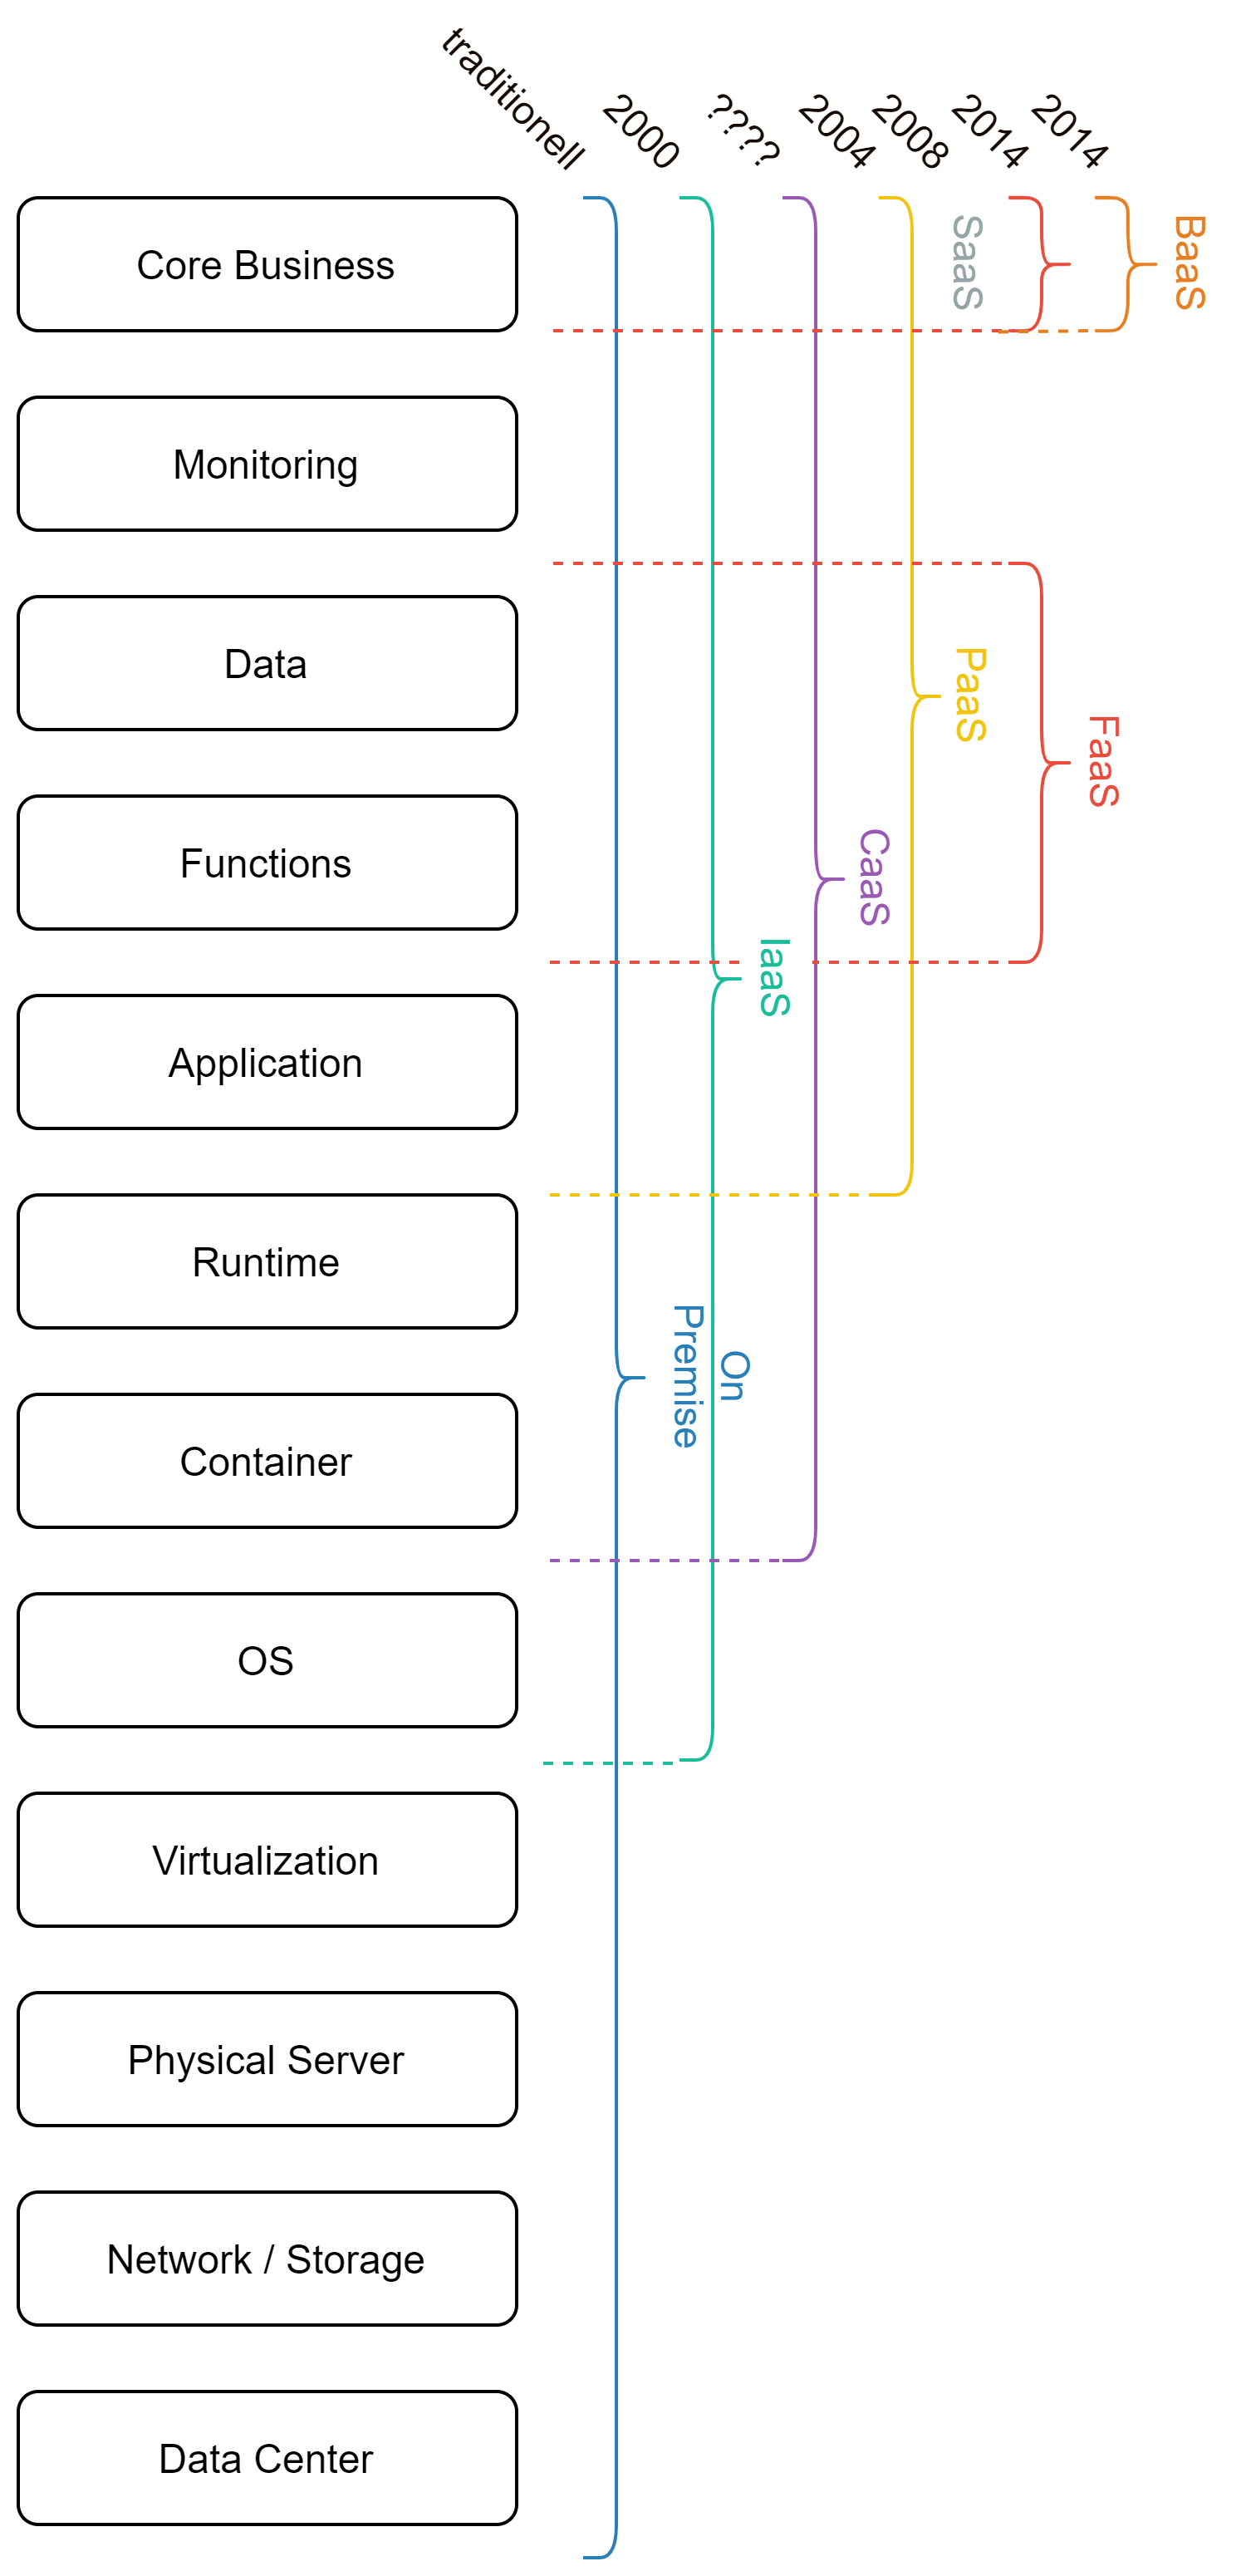
\includegraphics[angle=90,width=1\textwidth]{serviceModels}
\end{figure}
Neben den bereits genannten Service Models IaaS, PaaS und SaaS gibt es jedoch noch weitere, welche sich im Laufe der Zeit etabliert haben. Abbildung ~\ref{fig:cloudComputingConcepts} gibt einen Überblick hierüber. 


\subsection{Function as a Service}
Function as a Service (FaaS) ist ein sogenanntes \glqq Serverless\grqq{} Cloud-Computing Konzept, welches erstmals 2014 von AWS mit Lambda Functions als Preview Release und schließlich 2015 zur kommerziellen Nutzung zur Verfügung gestellt wurde \footnote{https://docs.aws.amazon.com/lambda/latest/dg/lambda-releases.html}. Es kann nach IaaS und PaaS als ein weiterer Schritt in der Entwicklung des Cloud Computings gesehen werden, welcher das Management von Infrastruktur, Servern und Ressourcen weg von dem Entwickler nimmt und hin zu dem Cloud-Anbieter delegiert. Ein knappes Jahr später, 2016, traten Microsoft mit Azure Functions, Google mit Google Cloud Functions und IBM mit OpenWhisk in den bis dahin von Amazon dominierten Markt ein. Mittlerweile gibt es eine vielzahl an Open-Source sowie proprietären Anbietern, welche um die Gunst der Kunden werben und einen stetigen Wettbewerb aufrecht erhalten. Ein ausführliche Übersicht über die jeweiligen Anbiter findet sich online von der CNCF \footnote{https://github.com/cncf/wg-serverless}\\\\
Da es sich mit FaaS und Serverless um eine noch recht junge Technologie handelt gibt es zu diesem Konzept keine offiziell dokumentierte Definition. bsp. von NIST o.ä., in der Literatur, wie es beispielsweise beim Cloud-Computing \cite{mell2011nist} der Fall ist. Die Anbieter sind sich jedoch über die Funkitionalität von FaaS größtenteils einig, was das Spektrum an Funktionalitäten anbegeht. So definiert Microsoft Azure Functions als: \glqq [...] event-driven serverless compute platform that can also solve complex orchestration problems. Build and debug locally without additional setup, deploy and operate at scale in the cloud, and integrate services using triggers and bindings. \grqq{} \footnote{https://azure.microsoft.com/en-us/services/functions/}. Hiermit beschreibt der Anbieter bereits die Kernfunktionalitäten von FaaS und drückt den Kerngedanken hinder FaaS aus. Das Konzept soll genutzt werden können, um bei dem Auftreten eines zuvor definierten sog. Triggers auf ein Event aus der eigenen Applikation oder der des Abieters reagieren zu können. Dabei stellen die meisten Anbieter wie Google, Azure oder AWS neben einem einfachen event-basierten HTTP-Trigger oder widerkehrenden zeitbasierten Triggern noch weitere, an die jeweilige Infrasturktur des Anbieters angepasste, Trigger zur Verfügung. Diese ergeben sich meist aus den BaaS Angeboten, hierzu mehr in \textit{Abgrenzung von FaaS zu Serverless}, welche in Form von Datenbank Triggern bei einer CRUD-Operation, dem Anlegen eines Nutzers oder der Integration mit einem Push-Notification Service [AWS SSN, Google Pub/Sub etc.] auftreten können.\\
\begin{figure}[H]
\caption[FaaS Programming Model nach OpenWhisk]{\footnote{http://openwhisk.apache.org/documentation.html}}
\label{fig:openWhiskProgrammingModel}
\centering
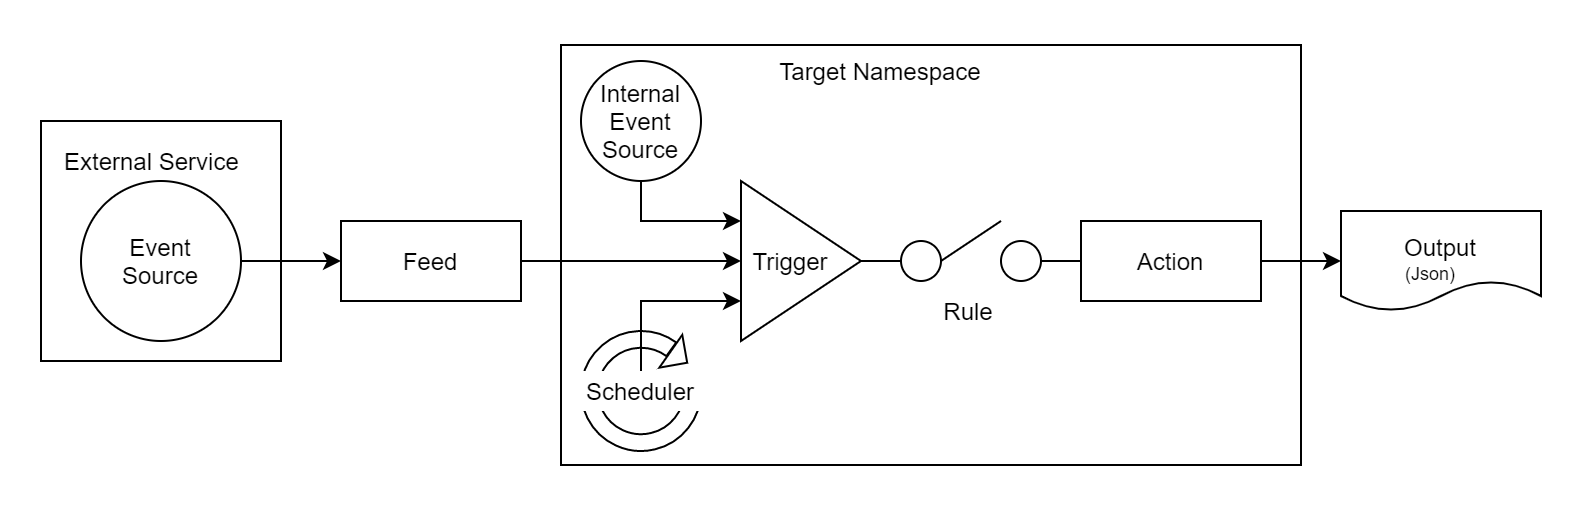
\includegraphics[width=1\textwidth]{ProgrammingModel}
\end{figure}
Abbildung ~\ref{fig:openWhiskProgrammingModel} gibt hierbei eine Übersicht über die verscheidenen Event-Trigger, welche derzeit bei den großen, proprietären Anbietern (AWS, Google, Microsoft) existieren. Da hinter OpenWhisk mit IBM eine großes Unternehmen steht, wird dieses Modell in der Literatur häufig als Referenz in Bezug auf die anderen Anbieter verwendet. Es kann angenommen werden, dass andere Abieter ein ähnliches Konzept bei ihrer FaaS Architektur verfolgen, da Apache OpenWhisk in einer großen Cloud (IBM) bereitgestellt wird \cite{van2019spec}. Eine weitere fundamentale Eigenschaft ist die erwähnte Skalierbarkeit, welche nach dem sog. \glqq Pay Per Use\grqq{}-Modell abgerechnet wird. Gemeint ist hiermit, dass der Kunde nur das bezahlt was er auch wirklich verbraucht hat, wobei die Verrechnung extrem granular nach genutzten Ressourcen und gelaufener Zeit erfolgt. Der Kunde bezahlt daher nicht für die benötgten Ressourcen, wie er es bei PaaS (wobei es hier variierende und bereits granularere Modell gibt) oder IaaS der Fall ist, sondern nur für die tatsächlich genutzten Ressourcen. \\\\
\textcolor{blue}{Grundsätzlich ist zwar der Preis der für das Laufen einer einminütigen Funktionsaussführung verglichen mit dem Laufen des selben Codes auf einem von den Ressourcen her ähnlich bestückten PaaS-Server günstiger \cite{jonas2019cloud}, jedoch der Anwendungszweck ein ganz anderer. Während mit PaaS Anwendungen bedient werden, die eine dauerhaft hohe Nachfrage erfahren, sollen mit Funktionen primär einfache stark frequentierende Aufgaben geläst werden, bei denen der Nutzer nur für die Ressroucen bezahlen muss die die Funktion bei dem Aufruf nutzt und nicht für jene die ohen einkommende Aufrufe provisioniert wurden.} \\\\
Ein weiterer wichtiger Punkt, welcher sich auch bei anderen Anbietern findet, ist in der Definition von OpenWhisk zum einen mit \glqq[...] you can focus on building amazing and efficient applications [...]\grqq{} und zum anderen mit \glqq  developers write functional logic [...] in any supported programming language, that can be dynamically scheduled [...]\grqq{}\footnote{http://openwhisk.apache.org/}. Ersteres meint die Abstraktion der Infrastruktur, welche dem Nutzer zum Bereitstellen von lauffähigem, skalierbaren, sicheren Backend-Code nicht bekannt sein muss. Die automatische Skalierung und optimale Verteilung von Ressourcen obliegt der Hoheit des Anbiters, und ist dem Nuzter nicht zugänglich, zumindest bei den proprietäre Anbietern. Letzteres ist zwar keine einzigartige Eigenschaft von FaaS, da dieses Konzept beriets lange bekannt ist und auch bei der Microservice-Enticklung häufig zum Einsatz kommt, jedoch ist die Auswahl aus vielen verschiedenen Programmiersprachen wie Java, Go, Javascript (Typescript), Python, PHP usw. (abhängig von dem jeweiligen Anbieter) unter dem Gesichtspunkt der direkten Nutzung zu sehen. Es muss keinerlei zusätzliches Setup oder andere Konfigurationen in der Umgebung vorgenommen werden, da dies der Anbieter übernimmt. Er kümmert sich um Patches und das Upgraden auf die aktuellste Version, was dem Entwickler ein großes Maß anflexibilität bei der Entwicklung der Anwendung einräumt. Eine weitere häufig in der Literatur referenzierte Defninition ist \cite{fowler2018serverless}, von Mike Roberts, welche die Beschreibung von AWS Lambda näher erläutert und im groben die oben genannten Punkte wiedergibt. \textcolor{blue}{Natürlich sind diese Eigenschaften mit einem gewissen Venodr Lock-In \textcolor{red}{dieser jedoch weder als schlecht noch gut zu bewerten ist und vielmehr nüchtern auf seine Vor- und Nachteile anasystiert werden sollte.} verbunden, da dieser Enstcheidungen über die Infrastruktur trifft, mehr dazu in \textit{Potentiale und Herausforderungen}.}\\\\
Abbildung ~\ref{fig:FaaSBaaSExample} verdeutlicht hierbei noch einmal die Wirkungsweise von FaaS. Oben rechts ist der Funktionspool zu sehen, welcher bei dem jeweiligen Cloud Provider steht und in welchen der Entwickler seine Funktionne lädt. Wird eine Funktion von einem Client aufgerufen, so wird bei Aktivierung eines Triggers eine Kopie der jeweiligen Funktion instantiiert und alle mit diese Funktion verbundenen Abhänigkeiten geladen (bspw. benötigte Module). Je nachdem wie frequentiert die Funktionen von den Clients angefordert werden, werden die vorhandenen Instanzen automatisch von dem Provider 
\begin{figure}[H]
\caption{Anwendung mit FaaS und (P)BaaS, angelehnt an \cite{shafiei2020serverless}}
\label{fig:FaaSBaaSExample}
\centering
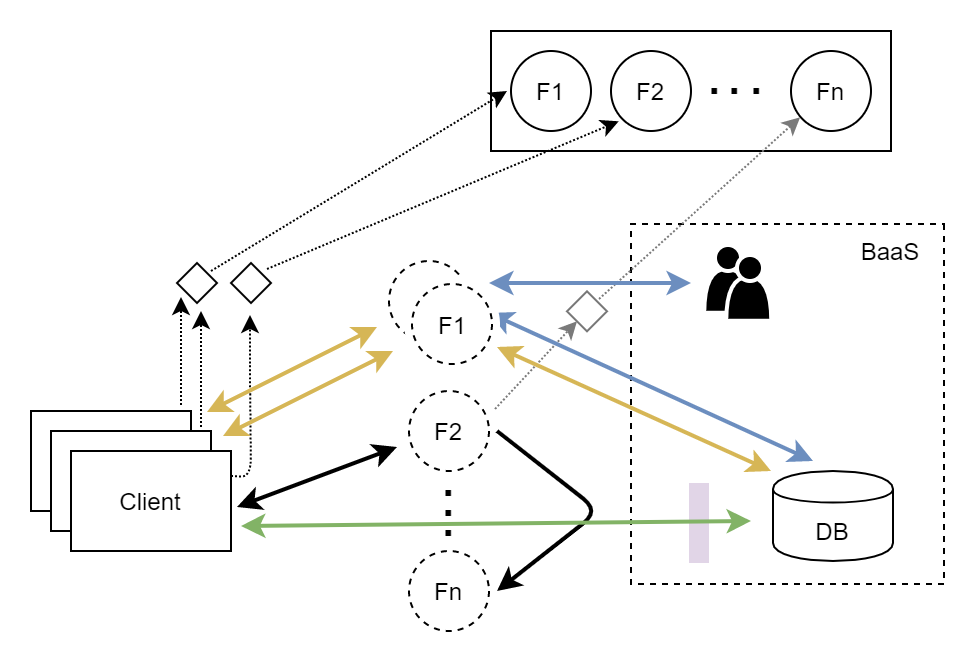
\includegraphics[width=1 \textwidth]{FaaS}
\end{figure}
hochskaliert, um den eingehenden Anfragen gerecht zu werden. Hierbei kann die Funktion eine Aufgabe direkt ausführen und das Resultat an den Client zurückgeben, oder wie bei F1 auf die im hintergrund laufende BaaS Infrasturktur zugreifen. Diese reicht von einfachen Datenbankabfragen bis hin zu anlegen eines neuen Nutzers etc. Limitiert werden die Möglichkeiten hierbei lediglich von dem Service-Ökosystem des jeweiligen Anbieters. Genauso ist es natürlich möglich Funktionen sich gegenseitig aufrufen zu lassen oder direkt mit BaaS-Servicen zu interagieren, siehe \textit{Abgrenzung von FaaS zu Serverless}. \\\\
Um FaaS besser und einheitlicher definieren zu könne und damit einen plattformübergreifenden Standart zu schaffen, wird in der Industrie und Forschung das Verlangen nach einer Referenzarchitektur, wie sie beispielsweise für das Cloud oder Grid Computing vorhanden ist \cite{liu2011nist}, \cite{foster2003grid} lauter. Die Abwesenheit einer solchen Architektur behindere die Etablierung von Best-Practices, Design Pattern und einen genaueren Überblick darüber zu erhalten, wie sich das Feld rund um Function as a Service entwickele \cite{leitner2019mixed}. Erste Vorschläge wie die Referenzarchitektur von FaaS aussehen könnte, haben sich mit \cite{van2019spec} durch die über die Jahre, von 2016 an, gestiegenen Popularität von Faas in der Forschung und der Literatur bereits herausgebildet. War hier die Thematik bis 2016 nicht addressiert worden, so stieg die Präsenz von hier an kontinuierlich bis 2019, in Journals, Konferenzen und Workshops an \cite{Yussupov2019_SystematicMappingStudyFaaS}. \\\\


\subsection{Abgrenzung von FaaS zu Serverless}
Serverless-Computing, oftmals auch als Serverless bezeichnet, ist eine Teildisziplin des Cloud-Computings, welche sich aus der Virtualisierung von Rechenleistung, Speicher und Netzwerken aus entwickelt hat \cite{jackson2018investigation}. Wie so häufig ist die Abgrenzung bzw. die Unterscheidung bei sich neu entwickelden Technologien nicht ganz einfach. Zunächst stand Serverless für Anwendungen welche teilweise oder komplett auf Drittanbieter zurückgriffen, auf sog. Backends as a Service (BaaS) [siehe Abbildung. ~\ref{fig:serverlessBaaSandPaas}], um serverseitige Aufgaben wie Datenbankabfragen, Nutzerverwaltung o.ä. zu regeln \cite{fowler2018serverless}. \\\\
Mit FaaS wurde das Serverless-Konzept dahingehend erweitert, dass die Serverlogik nicht mehr vollständig von einer dritten Partei zur Verfügung gestellt wird, sondern vom Entwickler selber implementiert werden kann. Serverless ist dabei eines der in den letzten Jahrne häufig genutzten Buzzwords in der IT, wobei der Begriff an sich etwas anderes suggeriert, als das was damit tatsächlich gemeint ist. Der Begriff impliziert die Abwesenheit von Servern, wobei damit lediglich eine Verschiebung der Zuständigkeiten einher geht. Entwickler einer \glqq Serverlosen\grqq{}-Anwendung bspw. mit FaaS, müssen sich nicht mit den operationellen Tätigkeiten wie dem \textit{Provisioning}, Monitoring, der Wartung der Infrastruktur, der Skalierbarkeit dieser und der Robustheit des Systems befassen \cite{baldini2017serverless}. Jedoch geht mit der Abgabe an Zuständigkeiten auch ein gewisser Vendor Lock-In einher, wobei die Anbeiter darauf achten, das mit FaaS eine möglichst große Zahl der in ihrem Service-Ökosystem vorhandene Services genutzt werden \cite{kritikos2018review}. Es sollen möglichst viele der bereits im vorherigen Abschnitt vorgestellten Trigger bei dem Bau von Anwendungen genutzt werden. \\\\
Function as a Service ist somit zum Großteil aus dem Event-Driven Computing, welches vor allem bei der UI-Entwicklung genutzt wird, abgeleitetes Konzept, welches Serverless-Computing adaptiert hat. Nichts desto trotz wird der Begriff Serverless in vielen Fällen, laut \cite{leitner2019mixed} in 58\% der Fälle, mit FaaS gleichgesetzt, was eine Abgrenzung erschwert. Abbildung ~\ref{fig:serverlessBaaSandPaas} verdeutlicht in welcher Beziehung die unterschiedlichen Konzepte stehen. 
\begin{figure}[H]
\caption{Serverless Concept, including FaaS and BaaS}
\label{fig:serverlessBaaSandPaas}
\centering
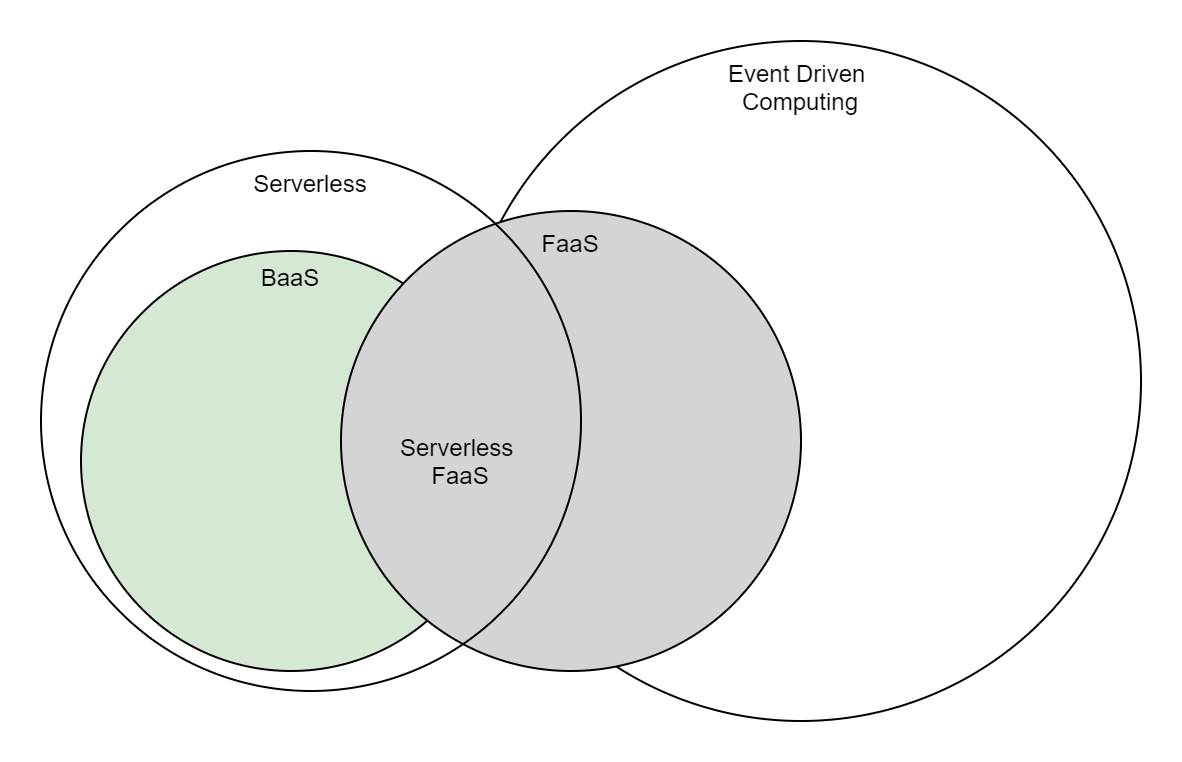
\includegraphics[width=1\textwidth]{Serverless}
\end{figure} 
Besteht eien Anwendung in der Folge lediglich aus den zwei \glqq serverlosen\grqq{} Komponenten, FaaS und BaaS, so ist häufig die Rede von einer \glqq pure serverless\grqq{}, also einer Anwendung, deren operationeller Teil vollständig an einen Cloud-Anbieter ausgelagert wurden und einer \glqq hybrid serverless\grqq{} Anwendung unterschieden \cite{leitner2019mixed}. Bei letzterem fungieren die Kunktionen häufig als sog. \glqq Glue\grqq{}, der meisten zeitlich variierend Aufgaben übernimmt, da IDLE-Zeit, wie man sie aus IaaS oder PaaS kennt, nicht berechnet wird.\\\\Nun mag der ein oder andere argumentiern, das ein Großteil der infrasturkurellen Aufgaben auch bei PaaS von dem Cloud-Anbieter übernommen werden, womit er natürlich recht hat. FaaS geht an dieser Stelle jedoch noch einen Schritt weiter. Bei Paas werden vorgefertigte \textit{Packages} einer Anwendung auf der Runtime der entsprechenden Plattfrom bereitgestellt, womit sich die Entwickler immer noch im die Anwenungsstruktur kümmern müssen \cite{kaplan2019framework}. In FaaS hingegen wird dieser Teil übernommen und der Entwickler konzetriert sich lediglich auf die Business logik und die jeweiligen Event-\textit{Trigger}. \\\\
Zuletzt soll noch auf einen weiteren Punkt, \glqq NoOps\grqq{}, eingegangen werden, der oft mit Serverless gleichgestellt wird. Es wird zwar durch die Übernahme des Loadbalancing, der automatischen Skalierung, Sicherheitsaspekten und Patches ein Großteil der Wartung ausgelagert, jedoch ist dies nicht mit der Annahme des Wegfalls der Operations von DevOps gleichzusetzten, wie suggeriert wird \cite{fowler2018serverless}. Es obliegt weiterhin den Entwicklern qualitativ hochwertigen Code zu schrieben und diesen in der Cloud-Umgebung zu testen, um dessen Performanz sicherzustellen. Die Komplexität entfällt daher nicht vollkommen, sondern verlagert sich zu einem gewiessen Teil \cite{eivy2017wary}. \textcolor{red}{Schaut man sich beispielsweise AWS an, so muss eine vielzahl an Konfigurationen vorgenommen werden. Zwar kann später eine vorhanden auf alle Funktionen angewendet werden, jedoch ist diese in der Folge von essentieller Bedeutung in einer riesigen \glqq Multitennacy\grqq{}-Umgebung.}\\\\% however, developers of serverless applications do not have to deal with any operational management with respect to provisioning, monitoring, maintenance,scalabilityandresilienceoftheserverstheapplicationisdeployedon \cite{baldini2017serverless}


\subsection{Potentiale und Herausforderungen}
Die im Folgenden aufgelisten Potential und Herausforderungen, denen sich Literatur und Anwender von FaaS gegenübersehen, sind zu Teilen dem Konzept selber, zu Teilen aber auch der Implementation der jeweiligen Anbeiter bzw. Open-Source Lösungen geschuldet. Es werden daher auf Seiten der Herausforderungen diese zunächst erläutert und falls in der Literatur bereits adressiert, vorgeschlagen Lösungen aufgezählt. Bei beiden, Potentiale und Herausforderungen, wird sowol Bezug auf FaaS als auch auf BaaS genommen, da diese beieden Kategorien in den meisten Fällen in Kombination genutzt werden bzw. architektionisch beding in Kombination genutz werden müssen [siehe Abbildung ~\ref{fig:serverlessBaaSandPaas} und \glqq statelessness\grqq{} Abschnitt \textit{Function as a Service}]. \\\\\\
{\normalsize \textbf{Potentiale}} \\\\
\textbf{Kosteneffizienz}\\
\\\\
\textbf{Time to Market / Lead Time Development}\\
\\\\
\textbf{DevOps}\\
\\\\
\textbf{Testing}\\
\\\\
\textbf{Optimale Auslastung von Rechenzentren}
Greener Computing \cite{shafiei2020serverless} \cite{fowler2018serverless}
\\\\
{\normalsize \textbf{Herausforderungen}} \\\\
\textbf{Vendor Lock-In}
Auch wenn diese Eigenschaft sowohl 
\textbf{Physische Lokation}\\
Eine weiterer Punkt ist die physische Lokation der Funktionen. Dadurch, dass es dem Provider obliegt, die Ressourcen seiner Infrastruktur optimal zu nutzen, entscheidet dieser auch auf welcher Node eine Funktion ausgeführt wird. Platziert der Provider in der Folge Funktionen, die eine hohe Datenabhänigkeit haben, physische weit voneinander entfernt, so wird sich dies auf die Performance der Anwendung auswirken und letztlich als Latenz bei dem Endverbraucher zu spüren sein \cite{shafiei2020serverless}. Es gibt zwar bereits bei vielen Anbietern, wie AWS, Microsoft oder Google die Möglichkeit die Region beziehungsweise ein sog. Cluster festzulegen, jedoch lässt sich damit die Lokation lediglich eingrenzen, aber nicht rechenzentren-genau festlegen. Mit der Performance von \glqq serverful\grqq{}-Applikationen kann damit nicht gleichgezogen werden \cite{shafiei2020serverless}. \\\\
\glqq \textbf{Serverless}\grqq{}\\
Es ist an dieser Stelle zwar relativ trivial, trotz alledem ein Nachteil verglichen mit Lösungen wie PaaS oder IaaS. Die Rede ist von dem Verlust der serverseitigen Optimierung. Wie bereits durch den Namen deutlich gemacht, existieren die Server für den Nutzer nicht bzw. hat er bei einer auf BaaS basierenden Softwarelösung keine Kontrolle über das Backend. Er kann lediglich die Datenbanken, Objektspeicher oder Authentifizierung an die Struktur seiner Daten anpassen und über \glqq Regeln\grqq{}Zugriffsbeschränkugen umsetzen. Die Services sind von dem jeweiligen Vendor vorgegeben und können bspw. nicht nach dem \glqq Backend For Frontend\grqq{}-Muster \footnote{https://samnewman.io/patterns/architectural/bff/} auf die entprechenden Client-Typen, wie Tablet, Mobile-Phone oder Desktop angepasst werden. Es existieren von jeder Sorte (Datenbanken, Objektspeicher, Authentifizierung usw.) nur eine Version auf welche man beschränkt ist. Jegliche benutzerdefinierte Logik muss daher in den Client ausgelagert werden, da es nicht auf backendseitig implementiert werden kann \cite{fowler2018serverless}. Mit FaaS kann dieser Effekt gemindert werden, indem ein leichtgewichtige Logik in form von Funktionen serverseitig umgesetzt wird. Hierbei erfolg die Interaktion mit den unterschielichen BaaS-Servicen über die vom Anbieter beschränkten Trigger [siehe Abschnitt \textit{Function as a Service}]. \\\\
\glqq \textbf{Statelessness}\grqq{}\\
Mit der \glqq statelessness\grqq{}, also der Zustandslosigkeit von Funktionen, geht eine weitere Problematik von FaaS einher. Der Kern von Anwendungen ist es Aufgaben zu lösen, wofür viele verschiedene Schritte von Nöten sind, welche sinnvoll miteinander verbunden werden müssen. So ist es auch bei dem funktionsbasierten Aufbau von Applikationen wichtig, dass diese untereinander kommunizieren können und den Programmstatus voneinander abfragen können, ohne das es zu Inkonsistenzen kommt. Bedingt durch die kurze Laufzeit der Funktionen ist es essentiell, dass auch der Austausch in entsprechender Geschwindigkeit erfolgt. Wie in einem Report von Berkeley \cite{jonas2019cloud} herausgearbeitet, erweist sich das schnelles und exaktes \glqq State-Sharing\grqq{} jedoch immer noch als problematisch dar, betrachtet man die Geschwindigkeit von \glqq Serverless\grqq{}-Anwendungen im Vergleich mit \glqq Serverful\grqq{}-Anwendungen. \\\\
Grund hierfür sind die von den Anbietern zur Verfügung gestellten BaaS-Lösungen für das persistente Speichern des Programmstatus. Objektspeicher der verschiedenen Anbieter (AWS S3, Google Cloud Storage, Azure Blob Storage) sind zwar nicht teuter sehr teuter wenn es um das Speichern mehrerer GB geht, jedoch sind die Kosten beim Zugreifen auf die Speicher hoch und die Latenzzeiten von bis zu 20ms zu hoch \cite{jonas2019cloud}. Die Key-Value-Speicher der Anbieter sind in diesem Falle die bessere Wahl, da ihre Ansprechzeiten mit 8 - 15ms geringer sind, jedoch sind sie, bezogen auf ihre Input/Output Operationen pro Sekunde, deutlich teurer als die der Objektspeicher. \\\\
Neben dem schnellen Informaitonsaustausch der Funktionen mit einem externen Speichermedium, kann es bei einer Kopplung von Funktionen aus performancetechnischen Gründen sinnvoller sein, den aktuellen Programmstatus direkt and die nächst Funktion weiter zu geben. Wie zuvor bei der \textit{physischen Lokation} der Funktionen erwähnt, ist es wahrscheinlich, dass Funktionen nicht auf der selben Node gestartet werden. Der Loadbalancer des jeweiligen Providers entscheidet je nach Auslastung der Infrasturktur, auf welcher Node eine Kopie der Funktion ausgeführt wird. Auch wenn im Idealfall die Weitergabe des \glqq application states\grqq{} schneller ist als der Zugriff auf ein externes Speichermedium, so wird dies durch \glqq Startup-Latencies\grqq{}und physischer Distanz wieder relativiert. Um dem entgegenzuwirken schlagen Shafiei et. al. \cite{shafiei2020serverless} vor, mit einem \textit{Dependency-Graphen} miteinander verwobene Funktionen zu kennzeichnen und direkt bei dem initialen Aufruf einer Funktion mögliche Folgefunktionen zu starten. \\\\
Würde man dem Nutzer die Möglichkeit geben zu bestimmen auf welcher Instanz (Node) eine Funktion laufen soll, so das Konzept von FaaS damit untergraben werden (siehe \textit{Optimale Auslastung}). Es würde dazu führen, dass erneut Kapazität zurückgehalten wird, über welche der Provider nicht mehr frei verfügen könnte. 
\begin{figure}[H]
\caption{Dependency Graph nach \cite{shafiei2020serverless}}
\label{fig:dependencyGraph}
\centering
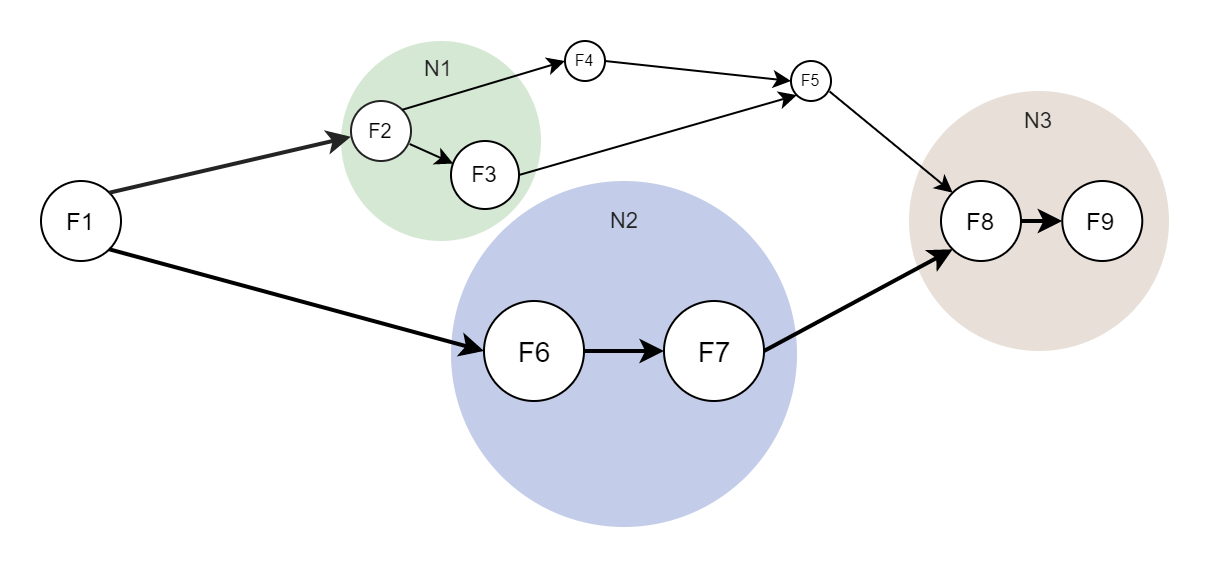
\includegraphics[width=1\textwidth]{DependencyGraph}
\end{figure} 
Wenn jeder Nuter bestimmen könnten auf welcher Node, bspw. Node-X, seine Funktionen laufen sollen, um den Progrmamstatus mit so wenig physisch bedingter Latenz wie möglich weiterzugeben, so wäre eine optimale Auslastung nicht mehr garantiert. Der Provider müsste stets Kapazität von Node-X zurückhalten und könnte sie nicht für andere Nutzerfunkitonen freigeben. Er muss stets einen Teil der Kapazität von Node-X zurückhalten, für den fall dass inaktive, aber der Node zugeteilte Funktionen aufgerufen werden. Mit einem \textit{Dependency-Graphen} wie in Abbildung ~\ref{fig:dependencyGraph} zu sehen würde dieses Problem umgangen werden. Der \textit{Load-Balancer} des Anbieters könnte unbeinträchtigt die Funktionen wie gewohnt je nach Auslastung auf freie Nodes verteilen, da er die korrelierenden Funktionen \glqq gleichzeitig\grqq{} starten kann. Da die Latenzen beim Starten eines Services erheblich höher sind, wobei die Programmiersprache dies zusätzlich beinflussen kann \cite{manner2018cold}, als jene durch die Lokation bedingt \cite{aditya2019will} \cite{jackson2018investigation}, würde deren Eliminierung die Weitergabe des \textit{States} erheblich beschleunigen. \\\\
Generell betrachtet könnte die Geschwindigkeit der Kommunikation von Funktionen untereinander beschleunigt werden. Verbindet man das ganze noch mit einem einfachen neuronalen Netz, um beispielsweise vorherzusagen mit welcher Wahrscheinlichkeit Funktion zwei (F2) im Vergleich zu Funktion sechs (F6) angesprochen wird, so könnte die Performance sogar noch ressourcenschonender auf Seiten des Cloud-Providers gestaltet werden. Zunächst käme es entweder zu einer höhreren Belastung, sollte man zu Beginne alle Funktionen starten oder zu einer höheren Latenz, sollte man die Funktionen einzeln starten und aus dem sich ergebenden Verlauf lernen. Nach einer kurzen Lernphase würde die Auslastung der Infrastruktur jedoch erhöht werden. \\\\
\glqq \textbf{Multitenancy}\grqq{}\\
Obgleich das Konzept von FaaS darauf beruht, dass der Anbieter eine Vielzahl von Funktionen verschiedener Kunden steuert und pflegt, so soll sich jeder Kunde fühlen, als sei der der Einzige. Allerdings stellt dies die Betreiber der Plattformen vor weitere Herausforderungen, da sie die Ressourcenisolation sowie Zugriffsbeschränkugen zuverlässig gewährleisten müssen. Dies ist jedoch leichter gesagt als getan, da es teilweise nicht nur von dem Provider selber, sondern auch von der richtigen Konfiguration der Sicherheitseinstellungen der Nutzer \footnote{https://awsinsider.net/articles/2017/06/20/voter-data-leak.aspx}, \footnote{https://searchsecurity.techtarget.com/news/450422962/Another-AWS-cloud-data-leakage-due-to-misconfiguration} abhängt, ob die Daten unzugänglich für Dritte sind. \\\\
Obwohl Anbieter wie AWS Mittlerweile erfahren genug sein sollten, dass solche Probleme nicht mehr zu erwarten sind \cite{fowler2018serverless}, ist weiterhin Vorsicht geboten. Es nichts an der Tatsache, dass auch sie sich mit Sicherheitsaspekten, der Robustheit und Performance ihrer Infrastruktur ständig weiter auseinadner setzten müssen. Kein Kunde darf die Daten eines anderen sehen, kein Fehler die Stabilität anderer Funktionen gefährden und kein plötzlich auftretender \textit{Spike} eines Kunden die Performance der Funktionen eines anderen beeinträchtigen. Das Zusammenspiel von RPCs und der Containersicherheit muss dauerhaft gegeben sein und durch sorgfältiges \textit{Security Managament} sichergestellt werden \cite{mcgrath2017serverless}.  \\\\
\textbf{Testing}\\
\\\\
\textbf{Cold-Starts}\\
\textit{Cold Starts} beziehen sich auf das Starten eines Containers, in welchem eine Kopie der benötigten Funktionen zur Verfügung gestellt wird. Ist eine Funktion lange nicht genutzt worden oder wird zum ersten Mal angesprochen, so muss für die Ausführung zunächst alles vorberietet werden. Vor allem bei sehr kurzen Funktionen stellen sie ein erhebliches Problem dar, da ihre \textit{Start-Up}-Zeit bis zu ein Zehnfaches der eigentlichen Ausführungszeit einnehmen kann \cite{shahrad2019architectural}. Ein Container muss auf einer Node gestartet werden und die Funktion, sowie deren Abhänigkeiten geladen werden. Die Zeit die es dauert, bis die Instanz bereit ist hängt dabei von verscheidenen Faktoren, wie der Programmiersprache, der benötigten Bibliotheken (\textit{Libraries}), der Größe der Funktion (menge an Code) und der Hardware \cite{shafiei2020serverless} \cite{jonas2019cloud} ab, auf der die Funktion instantiiert wird. Wird eine Funktion dabei sehr frequentiert aufgerufen, so halten die Plattformen diese Funktionen für eine gewisse Zeit vor (\glqq warm\grqq{}, bei AWS bis zu einer Stunde \cite{roberts2017serverless}, wodurch die Wahrscheinlichkeit eines erneuten \textit{Cold Starts} gegen Null tendiert. Bei Funktionen die hingegen nur einmal pro Stunde bemüht werden, sind die Folgen von \textit{Cold Start} deutlich häufiger zu spüren \cite{roberts2017serverless}. \\\\
Um dem entgegenzuwirken schlägt \cite{castro2019server} vor, eine Art stammzellen Container vorzuhalten. Diese würden für die unterstützten Programmiersprachen bereits instantiiert aber leere Container vorhalten. Diese Container sind nicht Kundenspezifischen und generisch nutzbar. Damit würden zwei der obene genannten Punkte, die Programmiersprache und die Hardware, welche die \textit{Startup}-Zeit der Funktionen negativ beeinflussen, eleminiert werden. Lediglich die größe der Funktionen und deren \textit{Dependencies} müssen noch geladen werden. \cite{ishakian2018serving} hat zudem gezeigt, dass mit der Erhöhung der Speicherkapazität die Zeit bis eine Funktion bereit ist einen \textit{Request} zu bearbeiten verringert werden kann. Kombiniert man dies mit dem Stammzellen-Ansatz, so wird das Laden des Programmcodes und der \textit{Libraries} beschleunigt. Natürlich kommt der zusätzliche Speicher nicht umsonst, jedoch liegt es in dem Fall bei dem Unternehemn zwischen den Mehrkosten und dem Performancezuwachs abzuwägen. \\
%Keep alive \cite{lloyd2018improving}
\newpage









\section{Guidline on Migration}
The below presented guideline for migrating parts of an existing microserive architecture to the relativeley new cloud-computing concept, Function as a Service, is structured as follows. At first the decision of migrating will be questioned, by challenging the motives of adopting this new technology and giving advice on when to migrate. Afterwards criteria for selecting the right service will be stated, which gear towards the possibilities that come along with FaaS. When a reasonable service has been found a provider needs to be identified which best meets the companys requirements. There are two types of providers that primarily differ in the service-ecosystem inherent to them and the degree of vendor lock-in. Whereas proprietary platforms like AWS, Azure or Google provide a great ecosystem of feature services and backend as a service offerings, open source frameworks like OpenWhisk, Fisson or Kubeless dedicate greater control to the developers. When implementing FaaS, the open source solution can be far more adjusted and configured to best suit an organisation needs. Next, impacts on the geral process of software developnet, the \glqq Dev\grqq{}-part in \textit{DevOps}, will be investigated. Changes on organisational structures regarding the deveopnet team, as well as effects on the CI/CD pipeline, challenges faced with local testing and the VCS will be addressed. With the development process covered, the guidline on migration will end with the operational part which will be taken into account. Alternations on the process of monitoring, maintenance and testing instances will be coverd and advice on coping with them will be given. \\\\
In order to better follow along the guideline, the subsequent section will give an overview of the prevailing microservice infrastructure. The development process as well as the operational tasks will be described, along with the underlying service-landscape.

\subsection{Zu grunde liegenden Architektur}
Um im weiteren Verlauf dieser Arbeit Aussagen über die nötigen Anpassungen und Auswirkungen auf das Unternehemen, die Entwicklung (Dev) selber, sowie die Kultur und den operationellen Teil (Ops) treffen zu können, soll zunächst der momentan vorliegende Aufbau beschrieben werden. Hierbei handelt es sich einfach gesagt, um die Entwicklung von Microservices, wobei momentan 31 Services in unterschiedlichen Versionen und Testinstanzen vorliegen. 

\subsection{Challenging the Decision}
Whereas migrating from a monolithic application to serverless, respectively function as a service, seems far more challenging, due to the assumed size and complexity of the application, migrating from a microservice-architecture can be challenging as well. With monolithic application, functionalities need to be identified in the first place and afterward be broken down into many small functional sections. Microservices, on the other hand, might already be small enough that they supply only certain functionalities but in some cases they do incorporate too many functionalities to be converted to functions right away. Nevertheless dealing with the issue of ousourcing the currently inherent state of services, as well as reducing dependencies and optimizing code remains. \\\\ %Before starting to introduce this new technology into the service landscape, it is essential to contrast the current state of the system with the desired state of the system. 
Before starting to introduce this new technology, the current state of the architecture as well as the desired state of the system need to be untangled. When a system is already composed of many small services, it is very likeley that the underlying infrasturcture consists of VMs or containers. Those containers often run in an PaaS environment and it is not possible to scale them to zero to free reserved computing capacity, in favour of other services to consume it. To do so or even to outsource the expense of provisioning services, managing the underlying infrasturcture and coping with operational tasks, such as monitoring, load balancing etc., Function as a Service can help to achive this desired state. On the other hand the restrictions that come along with the ease of development have to be traded off aginst its benefits. \\\\
In order to profit as much as possible of introducing FaaS, the services, which should be migrated, have to be inspected regarding depenencies, size, version, language and complexity. Starting with its dependencies, it is recommended to reduce them to a minimum, due to their effect on the star-up time of the container the function runs in \cite{manner2018cold}. Especially with Python, Nodejs and Java \cite{puripunpinyo2017effect} loading all dependencies required, which might again interconnect with other dependencies, will have an inpact on cold starts. The next issue which need to be addressed is state managemnt. As mentioned in section two, \textit{Benefits and Drawbacks}, there is no persistent state an application can rely on. There actually is persistent state in the container of a function, but whether an incoming request will hit a certain, running container, is unpredictable. When a service does not receive any request or is running for a long period of time, the provider will eventually kill its container to free capacity. In the case of AWS Lambda the current maximum amount of time, of a frequently called function untin it will be killed, is 45 minutes \footnote{https://aws.amazon.com/de/lambda/}. Later on, when comparing cloud providers with opne source framworks, there will be guideance on fining an appropriate solution to meet a companys purposes but for now the following must be considered. When using an open source framework like OpenWhisk, the external state management system can be covered with Redis or another low latency database, whereas using a cloud provider platform, one of its inherent database solutions will presumably be the best choice. If it is necessary to have full control over the performace and configuration of the databse, an open source framework has to be choosen. \\\\
Latency and frequency of a service will also decide upon its aptitude of beeing a candidat to be migrated to FaaS. If the service is called very frequent and experiences most of the time a very high traffic, the concept of Function as a Service will not be applicable to it \cite{jonas2019cloud}. Due a limit of concurrent running functions, that can vary between the different providers and frameworks, traffic can only be handled upon a certain amount. Moreover, the same application experiencing the same amount of traffic, once running on a FaaS platform and once running in a docker container in a PaaS environment, will be more expensive implemented with FaaS, than it will be with PaaS \cite{jonas2019cloud}. Therefore, services with various worklaods, having eventually high peeks and then some time of inactivity, are more applicable to the concept of serverless, then their counterparts. Latency should also not be a critical component due the before mentioned cold starts. Latency sensitive applications like trading platforms, which strongly rely on real time data, are not a suitable candidat for Function as a Service. \\\\
Another pitfall is the promise of not having to maintain, provision, scale or monitore the infrasturcture and thereby reducing complexity and operational tasks. On one side, the cloud provider will, to some extend, take care of load balancing, scaling functions up and down and providing monitoring solutions. On the other side, new complexity will appear in other areas. The issue of mono-repo and poly-repo arises, as discussed in a later section, as well as the necessity to learn the provieders DSL, accuire the skills to correctly configure security policies, interconnect function, define different triggers on functions, dealing with concurrency setting \footnote{https://docs.aws.amazon.com/lambda/latest/dg/configuration-concurrency.html} and many more aspects will add complexity in new fields. If the company aims at reducing infrasturctural complexities, then function as a service can support at the listed tasks, but when its main pupose is to reduce operational efforts, as often suggested with the term \glqq NoOps\grqq{} \cite{eivy2017wary}, FaaS, again, is not the right choice.\\\\
Lastly attention needs to be drawn to the programming language and lead time development. FaaS can provide a reduction in lead time development and time to market \cite{sewak2018winning} \cite{leitner2019mixed}, thanks to its small code base and rapid development. Developers are able to make changes, fix issues, test and finally deploy a new version to production in a view minutes. Prerequisite, even though this might sound trivial, is the platforms language support for the languaged used in the application or service. Despite the fact that many programming languages are already supported by the big cloud providers, application logic might have to be rewritten, if that specific laguage is not supported. The code also needs to be rewritten in case of verison incompatibility, when the version of the application is ahead of the version offered by the provider. 
\subsection{Choosing a suitable service}
git init && git add README.md && git commit -m "first commit" && git remote add origin https://github.com/gpitsystems/Bachelor.git && git push -u origin master

\subsection{Auswirkungen auf die Team-/ Entwicklungsstruktur}
Agile  / Dev Ops
%Other research has analyzed the role of cloud computing as an enabler for organizations to become more agile and adapt to changes [2] and how to organize IT functions when using cloud services [10, 47].\cite{benlian2018transformative}

% We suggest that new deployment of a function need to be prepared with the equivalent size of function instances compared to the current loads which will prevent delaying responsetimeinthecontextofconcurrentinvocations.Serverless framework with DevOps may enhance software development and continuous delivery through an agile function deployment and configuration as we will use multiple functions together with frequent changes. \cite{lee2018evaluation}


GIt abzuwägen, da verschiednen arten unterschiedliche VOr- und Nachteile haben. Rewiew (Peerreview bleibt gleich, auch dependency managament, da es von dem Kontext und der Sprache abhängt)
%Serverless influence: Serverless architecture affects the decision of how many code repositories to create. In case of monolithic architecture, the source code is tightly coupled and is usually stored in a single repository. Serverless architecture expects presence of multiple deployable units or functions that can be completely isolated from each other. Source code of these deployable units, for instance, of AWS Lambda functions, can be stored in multiple repositories with one repository per function approach or in one single repository for all functions. One more approach is to create several repositories, each of which will store multiple functions based on their purpose or domain field. \cite{ivanov2018implementation}
%Implementation ideas: VCS should be Git since it has very efficient branching model and team already has an experience with Git and GitLab. A number of created repositories should be defined based on the good practices of Serverless applications code maintenance.\cite{ivanov2018implementation}

% The projects we analyzed always had all their functions in the same repository. This is in fact much easier to manage by developers and maintainers \cite{brousse2019issue}

%As expected, the duplication of code is an issue encounteredinouranalysis. Halftheprojectsencountered this problem. As described in H2, the units of code are bigger than expected. Analysability may be an issue for serverless applications. \cite{racicot2019quality}

%Dependencies are managed in a repository: Serverless influence: Dependency management of Serverless functions has no differences with non-serverless project. The tools depend on the using language. Implementation ideas: All project dependencies and their versions should be defined and stored in VCS. \cite{ivanov2018implementation}

%However, we think that a serverless architecture does not have a positive impact on the code duplication in the case where a project uses multiple serverless functions. Because all functions have to be independent, we expect to find the duplication of libraries and helper functions. \cite{racicot2019quality} 

%Since the projects and the use cases are fairly small, it may be tempting for developers to put everything in the same unit and not to split the code base correctly. It may become an issue with small projects which are scaling more than the initial scope.  It does not seem like serverless technologies tend to be easy to modify \cite{racicot2019quality}

% \cite{fox2017status} stated, serverless is good for short-running, stateless and event-driven codes such as micro-services
Deployment /CI CD: 
% Multiple functions can requiretobedeployedatthesametimeiftheirinterface or behaviour changes. \cite{racicot2019quality}
% mono-repository versus multirepository (Potvin and Levenberg, 2016; Potencier, 2016; Cavale, 2016). Having only one repository per lambda can help to set up continuous integration tools (Amazon, 2017a). On the other hand, it is much easier to manage each functions of a project in a single repository, especially if all functions are only bound to a single project. \cite{racicot2019quality}

%Deployment: By observing Table I, someone would misjudge that the frameworks do not support function deployment at all. On the contrary, they do via the offering of appropriate CLIs. However, due to the modern way via applications are built with a rather agile development and provisioning lifecycle, we needed to examine if the frameworks could provide good or excellent support to this overall pipeline. In this respect, we can clearly see this support is really bad in overall, with only two frameworks offering a certain solution to the considered criteria. With respect to CI/CD, Sparta offers two respective solutions. The first relies on AWS CodePipeline11 while the second on a custom solution based on other AWS services. On the other hand, Serverless relies only on CodePipeline. In both frameworks, through the use of AWS CodeDeploy12, it is now possible to also gradually shift the traffic from an old to a new function version. Concerning versioning, again only Sparta and Serverless offer support for it mainly in the context of AWS Lambda. Which means that someone would have to lock-in to this platform to be able to realise this feature. We hope that this situation changes in the near future. \cite{kritikos2018review}


% 4.4.4 Deployment
% Fully scripted deployments
% Serverless influence: Serverless architecture influences a choice of cloud provider and deployment tool. Deployment tool should be scripted in a certain way.
% Implementation ideas: Deployment of Lambda functions can be done with CloudFormation, Terraform or Serverless Framework tool. Any of these tools can be run by GitLab CI.
% Auto deploy to the test environment after tests pass
% Serverless influence: Script triggering depends on CI pipeline tool and does not depend on the architecture of application. At the same time, if the team decides to keep all Lambda functions in separate
% CHAPTER 4. CURRENT STATE ANALYSIS 40
% repositories with their own deployment scripts, it can make the deployment of the project more cumbersome.
% Implementation ideas: Deployment stage of GitLab CI pipeline should be triggered only after the test stage was passed.
% Standard deployments for all environments
% Serverless influence: Serverless environment depends on cloud provider. How exactly functions will be deployed depends on the Serverless architecture. On-premises Serverless solutions such as Kubeless and OpenFaaS can help to avoid testing environment and vendor lock-in problems but they would also require resources on server maintenance nullifying time-saving benefits of third party provider usage.
% Implementation ideas: Infrastructure provisioning should be done with a help of IaC tools: CloudFormation or Terraform. The project should be deployed directly to the cloud but to different stages or even accounts.
% Database deployments
% Serverless influence: Serverless databases make database admin tasks unnecessary. Only schema changes or query changes are required. In case of NoSQL databases even schema changes are not required.
% Implementation ideas: DynamoDB database will be deployed to the cloud as all other services. It also does not require database schema migrations, because it is NoSQL DB. \cite{ivanov2018implementation}



Vorsicht bei der Anzahl der Funktioenn geboten, da sie sehr klein sind, gefahr höher dass mance Funktionen dupliziert werden, daher vielleicht eher Monorepo. Zudem leidet dann die Wartbarkeit des Codes darunter, da manche Funktionen mehrfach in leicht unterschielischer Weise vorliegen. Falls von den ähnlichen Funkitonen auch noch unterschiedliche Versionen existieren, so kann dies die Wartbarkeit zusätzlich erschweren \cite{racicot2019quality}.  
%  Factors that influence the modifiability are the amount of duplicated code, the complexity of the code units and the coupling between the modules. \cite{racicot2019quality}



Adopting serverless requires a different mental model, where systems are primarily constructed by composing pre-existing services, with FaaS often acting as the “glue” that brings these services together. FaaSofferstechnicalandbusiness-relatedadvantages, but managing and predicting deployment costs is difficult for larger applications. Further, tooling availability and maturity, especially related to testing and deployment, remains a barrier to entry. Finally, limited support for function sharing and the absence of a service ecosystem is seen as a challenge.  \cite{leitner2019mixed}

Um ein Aussage darüber treffen zu können, ob und in welchem Maße Anpassungen an der Team- bzw. Entwicklungsstruktur vorgenommen werden müssen, gilt es zunächst zu klären, wie die zu grunde liegende Unternehmensstruktur aufgebaut ist. Da diese Arbeit von einer bereits existierende Microservice-Architektur ausgeht, soll zunächst im Folgenden der organisatorische Aufbau dieser beschrieben werden. Im Nachhinein wird dieser noch einmal mit den entsprechenden Änderungen aufgegriffen, um eine bessere Aussage über die tatsächlich notwendingen Anpassungen treffen zu können.
Durch das neue Programmier-Paradigma wird den Programmierern automatisch ein neuer Aspekt auferlegt. Dadurch, dass die Funktionen einzeln nach Laufzeit und bezahlt werden, liegt es im interesse des Programmierers diese so performant wie möglich zu gestalten, um bei jedem Funktionsaufruf Ressourcen und Laufzeit einzusparen \cite{shafiei2020serverless}. 

\begin{figure}[h]
\caption{Referenzarchitektur Microservice-Entwicklung}
\centering
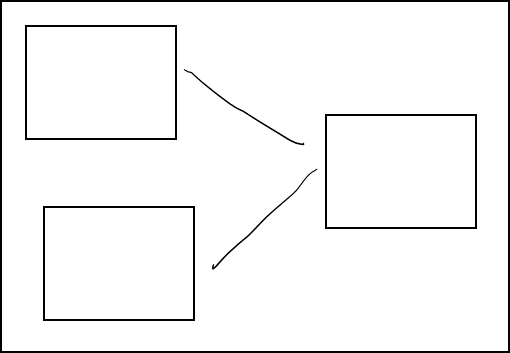
\includegraphics[width=0.5\textwidth]{test}
\end{figure}

\cite{van2019spec}
\cite{Yussupov2019_SystematicMappingStudyFaaS}
\cite{lee2018evaluation}
\cite{aws2020ManagingFunctions}
\\\\
Um provisioned concurrency festzulegen, sollte nachgesehen werden, wie häufig ein Funktion bzw. ein Service aufgerufen wird, und dementsprechend geschaut werden, wie viele Funktionsinstanzen immer vorrätig sein sollten. zudem sollte geprüft werden, wie lange ein Funktionsaufruf von dem Initialen Event bis zu seiner Response braucht, um zu schauen in wie weit dei Preformance durch die Nutzung einer alternativen Programmiersprache gesteigert werden kann. 
Eine weitere Möglichkeit bietet AWS mit Application Auto Scaling welches porvisioned concurrency erweitert ... \textcolor{green}{Target tracking scaling policy, welches provisioned concurrency automatisch napasst, je nach Nutztungsmetrik}
\subsection{Abwägung Open-Source und Cloud-Vendor}
Wie bereits im vorherigen Abschnitt beschrieben, 
OpenFaaS  
%OpenFaaS is a lightweight open-source framework which enables to build a serverless platform on top of Kubernetes and Docker Swarm. Serverless applications can be deployed on-premise or on any privateandpubliccloud. OpenFaaSconsistsofanAPIGatewaythatcanbeexposedtoanykind of event, such as services from AWS, Azure or open-source services, such as Minio [Min19] or MongoDBAtlas[Mon19a]. Furthermore,thedeploymentcanbeperformedmanuallythroughthe UIportalorautomatedusingtheOpenFaaS-CLIwithmanifestfilesfortemplatinganddefining functionsinYAMLformat.

Die Abwägung zwischen der Implementation von Function as a Service in der unternehmenseigenen Cloud bzw. Servern oder dem Outsourcen an einen proprietären Cloud-Vendor, sollte wohl überlegt sein, da hiervon in der Folge eine Vielzahl an Möglichkeiten und Restriktionen abhängt. \\\\
Entscheidet man sich für ersteres, also dem Aufbau einer privaten FaaS-Plattform so stehen hierfür, mit IBM Apache OpenWhisk, Fission, OpenFaaS oder Kubless, nahezu identisch viele Frameworks zur Verfügung wie bei den öffentlichen Vendoren. \textcolor{blue}{Schaubild CNCF Serverless Landscape ggf. einfügen.} Des Weiteren bietet dieser Weg, abgesehen von der Vielfalt an Frameworks mit wiederum unterschiedlichen Eigenschaften, die Möglichkeit die Größe der Funktionen oder die maximal zulässige Laufzeit eines Containers individuell anzupassen. Dies würde einerseits eine granularer Verrechnung der in Anspruch genommenen Ressourcen der einzelnen Bereiche oder Teams zulassen, zugleich aber auch ein Operations-Team verlangen, welches sich in das jeweilige Framework einarbeitet, die Plattform zu dessen Betrieb aufsetzt und die spätere Wartung dieser übernimmt. \cite{mohanty2018evaluation}.\\\\
Eine Alternative stellen proprietäre Lösungen von öffentlichen Cloud-Vendoren, wie beispielsweise Amazon Web Services (AWS) Lambda, Microsofts Azure Functions, IBM Cloud Functions oder Google Cloud Functions, bei welchen sich von Unternehmensseite aus niemand um die Wartung der Infrastruktur, die Skalierung der Services, die Behandlung von Fehlermeldungen o.ä. kümmern muss. Diese Aufgaben werden in der Folge von dem Plattformbetreiber übernommen. Natürlich sind diese Dinge in erster Linie Aufgabe des Plattformbetreibers, jedoch haben sie unmittelbare Auswirkungen auf das Unternehmen, sollten Probleme beim Skalieren von Funktionen oder dem Monitoring auftreten. Sollte dies der Fall sein, so sind die Entwickler von den bereitgestellten Debugging Möglichkeiten und Monitoring-Lösungen der Plattform abhängig um Probleme schnellstmöglich zu beheben, sollte dies die Plattform nicht tun. Daneben ist ein weiterer Punkt des Vendor Lock-Ins die von Anbieter zu Anbieter variierende Infrastruktur, welche ein einfaches Shiften von Funktionen erheblich erschwert. Zudem sind die Benutzung der Funktionen meist automatisch mit der Inanspruchnahme weiterer Services der Plattform, wie dem Message Queuing oder der Datenspeicherung, gekoppelt. \\\\
Dies hat sowohl Vor- als auch Nachteile. Ist man bei der Einrichtung der privaten FaaS-Cloud auf die unternehmensinternen Ressourcen beschränkt, so bieten die Cloud-Anbieter, neben den Restriktionen des Vendor Lock-Ins, in den meisten Fällen ein großes Ökosystem an weiteren Services, welche sich problemlos an die Funktionen anbinden lassen. Im Folgenden wird daher, auch wenn sich diese Arbeit hauptsächlich auf FaaS beschränkt, das Ökosystem der einzelnen Cloud-Anbieter kurz betrachtet, um einen besseren Überblick über deren zusätzliche Leistungen zu erhalten und eine fundierte Entscheidung treffen zu können.



\subsubsection{Vendoren-Analyse}
Ein weiterer Punkt bei der Migration von Teilen einer besehenden Architektur, in diesem Fall einer Microservice Architektur, ist die von dem Cloud-Vendor zur Verfügung gestellte Möglichkeit der Orchestrierung der Funktionen. Diese entscheidet darüber wie performant die Funktionen parallel ausgeführt werden können und wie groß der Runtime-Overhead der jeweiligen Plattformen dabei ist. Zudem spielt der Preis der hierfür anfällt eine nicht unerhebliche Rolle, da die sequentielle als auch die parallele Ausführung von Funktionen bei mittleren und großen Softwareprojekten häufig auftreten. \\\\
Wie bereits in \textit{Potentiale und Herausforderungen} unter \textit{Statelessness} erwähnt spielt bei der Kopplung von Funktionen die Weitergabe des Anwendungs- bzw. Funktions-\textit{States} und dessen Geschwindigkeit eine wichtige Rolle. Nur durch das richtige Zusammenspiel vieler Funktionen ist es möglich große Anwendungen zu bauen und komplexe Abläufe umzusetzen. Bei der Betrachtung der unterschiedlichen Hosting-Lösungen soll der Fokus auf die beiden am häufigsten genutzen proprietären FaaS-Lösungen \cite{leitner2019mixed}, AWS Lambda mit Amazon Step Functions und Microsoft Azure Functions mit Azure Durable Functions, gelegt werden. Die Seite der Open-Source Lösungen wird von IBM OpenWhisk, mit IBM Composer als Orchestrierungs-Lösung, vertreten.\\\\
\cite{lopez2018comparison} hat diese drei Frameworks genuaer untersucht und bei der sequentiell und parallele Planung sowie der Weitergabe des \textit{States} der drei Orchestrierungs-Tool erhebliche Unterschiede feststellen können. Vorab soll an dieser Stelle vermerkt werden, dass nur \glqq warme\grqq{} Instanzen für jegliche nachfolgende Tests genutzt wurden, um Ungenauigkeiten, durch variierende \textit{Cold-Start} Zeiten [siehe \cite{manner2018cold} und \cite{jackson2018investigation}], vorzubeugen. \\\\
In Bezug auf die Ausführung von aufeinander folgenden Funktionen, sequentielle Verarbeitung, erwiesen sich IBM's Composer und ASF als deutlich schneller im Vergleich zu ADF. So Betrug der Overhead, also die Zeit welche nicht zur Ausführung der Funtkion verwendet wurde, bei 40 hintereinander geschalteten Funktionen 1,1s für IBM Composer und 1,2s für AWS Step Functions. Azure Durable Functions brauchten hingegen für die selben 40 Funktionen ganze 8s. Bei weiteren Durchführungen mit [5, 10, 20, 40, 80] stellte sich jedoch heraus, dass IBM Composer die Orchestrierung von Funktionen nur bis zu einer Anzahl von 50 Stück unterstützt. Alles was darüber hinausgeht, müsste durch Orchestrierungs-Tool von Drittanbietern übernommen werden \cite{lopez2018comparison}. ADF und ASF sind wiederum in der Lage \textit{Workflows} festzulegen, welche über Tage und Monate lauffähig sind. \\\\
Die Evaluierung des Overheads bei parallel geschalteten Funtkionen wurde für ASF und ADF durchgeführt. Dabei wurde wieder mit 5 Funktionen begonnen und sich, wie oben beschrieben, bis auf 80 hochgearbeitet. Die Ergebnisse waren eindeutig. Bei einer Anzahl von 80 Funktionen hatten Azure Durable Functions mit einem durchschnittlichen Overhead von 32.1s fast das doppelte Volumen von AWS Step Functions mit einem durchschnittlichen Overhead von 18.3s. Die Ergbenisse legten zudem nahe, dass ASF zuverlässiger bei der Vorhersage des zu erwatenden Overheads ist als ADF. Microsofts Overhead stieg nicht immer gleichbleibend exponentiell an wie der von Amazon, was eine Prognose über das Verhalten erschwert.\\\\
Bei der Evaluierung für die Eignung von parallel geschalteten Funktionen viel IBMs Composer direkt zu Beginn aus dem Testportfolio heraus, da parallele Ausführungen nicht unterstützt wurden [stand 2018 \cite{lopez2018comparison}]. Mittlerweile [stand 2020] wird von Seiten IBMs die parallele Ausführung von Funktionen seitens Composer zwar unterstützt und gesagt, dass seitens Composer dies nicht auf eine bestimmte Anzahl von Funktionen beschränkt ist \footnote{https://github.com/apache/openwhisk-composer}. Allerdings wird explizit erwähnt, dass eine Limitierung gleichzeitig ausführbarer Funktionen Seitens OpenWhisk besteht, welche bei Überschreitung zu Fehlern führen kann: \glqq [...] many concurrent invocations may hit OpenWhisk limits leading to failures: failure to execute a branch of a parallel composition or failure to complete the parallel composition [...]\grqq{} \footnote{https://github.com/apache/openwhisk-composer}. Die derzeitige Limitierung gleichzeitiger Funktionen in OpenWhisk liegt bei 100 pro \textit{Namespace} \footnote{https://github.com/apache/openwhisk/blob/master/docs/}. \\\\
Zuletzt wurden die drei Orchestrierungs-Lösungen bezüglich der Weitergabe des \textit{Application-States} untersucht. Aufgrund der Begrenzung von ASF auf 32KB wurde bei den beiden anderen Lösungen die selbe Größe gewählt. Dieses mal wurden nur 5 sequentiell ablaufende Funktionen getestet. Die Grenze bei IBM Cloud Functions lag 2018 offiziell bei 1MB, liegt mittlerweile aber bei 5MB \footnote{https://cloud.ibm.com/docs/openwhisk?topic=cloud-functions-limits}. ADF hingegen ermöglich die Weitergabe von bis zu 60KB. Es zeigte sich, dass IBM Composer und AWS Step Functions bei der Ausführung ohne \textit{Payload}, jeweils einen Overhead von 175.7ms und 168.0ms hatten. Mit Payload betrug der Overhead in ms für Composer 298.4 und Step Functions 287.0, was eine Zunahem von 70\% darstellt [siehe Abbildung ~\ref{fig:orchestration}]. Azure Durable Functions stieß bei diesem Test deutlich hervor. Mit einem Overhead von 766.2ms ohne Paylod und 859.5ms mit Payload ist der grundlegende Overhead zwar deutlich höher als bei den beiden vorherigen, steigt unter Last aber nur um 12\% an \cite{lopez2018comparison}.
\begin{figure}[H]
\caption{Overhead bei 5 sequentiellen Funktionen mit einem Payload von 32KB, nach \cite{lopez2018comparison}}
\label{fig:orchestration}
\centering
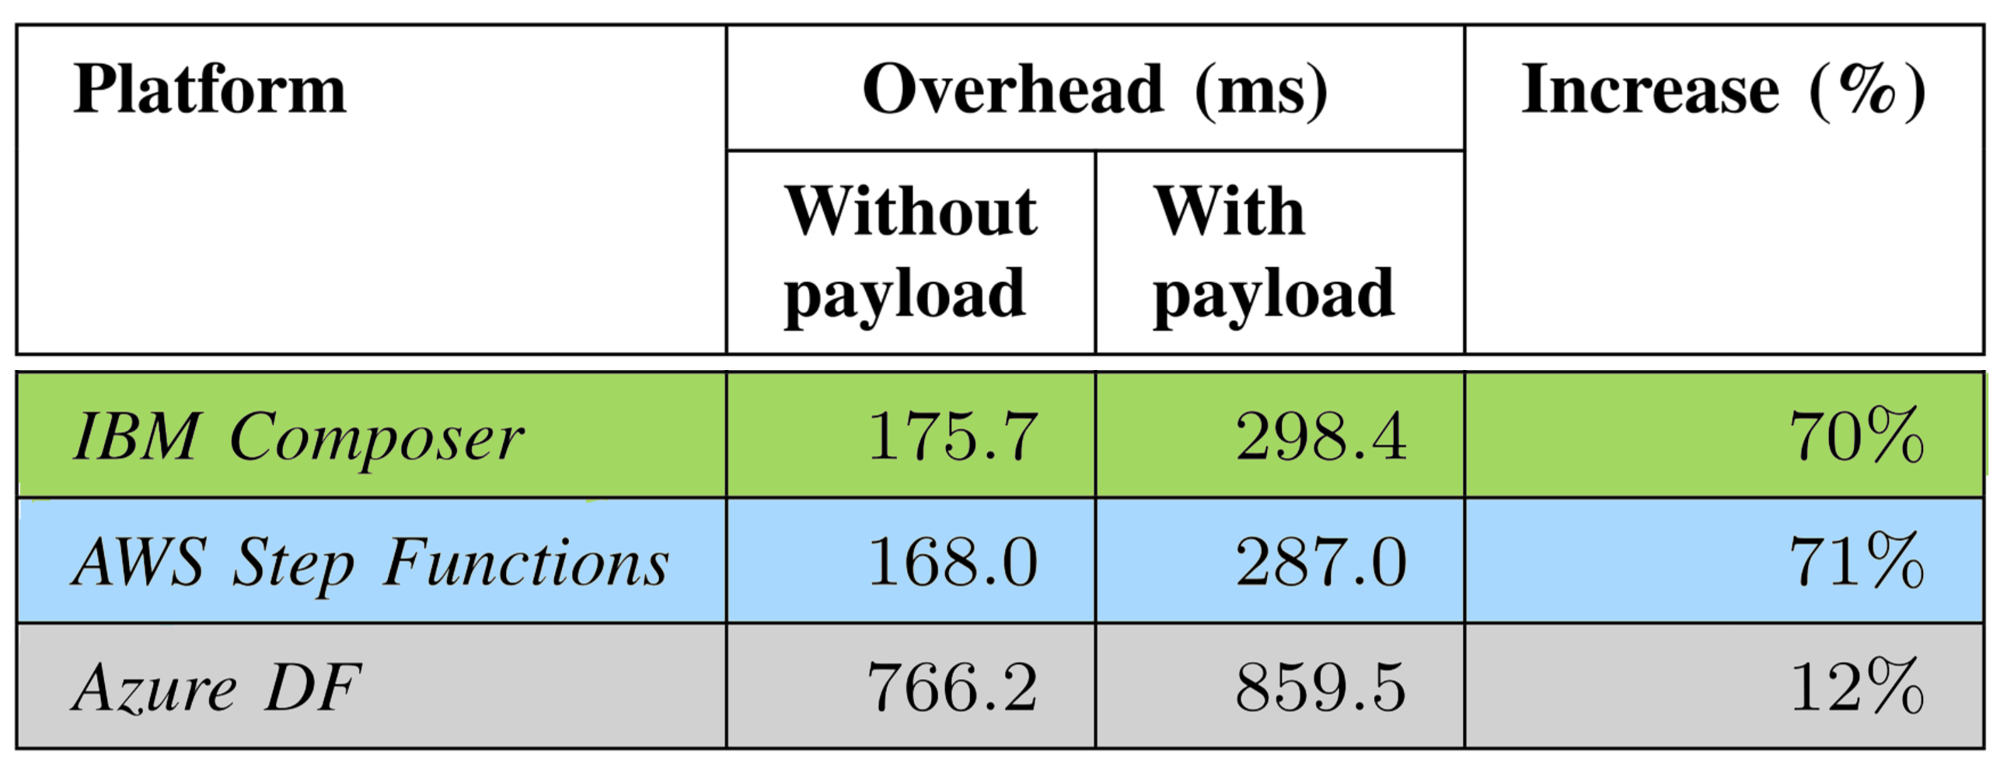
\includegraphics[width=1\textwidth]{Orchestration}
\end{figure} 
Anhand der durch Lopez et. al. gezeigten Ergebnisse lässt sich festhalten, dass AWS mit Step Funtion das ausgereifteste Orchestrierungs-Tool zur Verfügung stellt. Sowohl bei der sequentiellen als auch bei der parallelen Ausführung beitet AWS Lösungen für langlebige und kurzlebige Funktionskopplungen. Zudem ermöglicht die Limitierung des \textit{States} auf 32KB eine klare auskunft über die entstehenden Kosten zu geben. Hat man vor FaaS lediglich für leichtgewichtige Aufgaben zu nutzen, so spielt IBM Composer bei der Kopplung von bis zu 50 Funktionen seine Stärken aus und ist dabei geringfügig schneller als AWS. Für die Festlegung längerer Abläufe, welche auf das Laufen über Tage bis hin zu Monaten ausgelegt sind, ist Composer nicht geeignet \cite{lopez2018comparison}. Steht der Austausch des \textit{Application-States} zwischen Funktionen im Vordergrund und können höhere Latenzzeiten in Kauf genommen werden, bietet Azure mit einer Kapazität von 60KB eine Alternative zu AWS und IBM. Auch Abläufe die länger Zeit beanspruchen können mit ADF konfiguriert werden. Das Konzept von \textit{async/await} bei sequentiellen und \textit{fan-out/fan-in} \footnote{https://docs.microsoft.com/en-us/azure/azure-functions/durable/durable-functions-cloud-backup} bei parallelen Abläufen bietet zusätzlich eine etwas leichtere Umsetztung als AWS und IBM \cite{lopez2018comparison}.
%The orchestration component defines the sequence of tasks; all executions are automatically triggered, each step is tracked and retried in the case of error \cite{werner2018serverless}. AWS Step Functions Each step of an application is triggered, tracked and even retried when errors occur, assuring that applications execute as expected and in the correct order. To aid debugging and diagnostics, logs are kept for every step of the process. Figure 3 shows this process. An added benefit is that step functions can be created and deployed in code through the definition of a state machine using Amazon’s JSON-based States Language10. \cite{werner2018serverless}. 
Kein garantie, dass der folgende Funktionsaufruf auf die selbe bereits laufende Instanz einer Funktion trifft, welche dann wiederum auch zugriff auf dem im Memory gespeicherten State hat. Es ist daher notwendig, dass der Application-State extern gespeichert wird. Auf diesen sog. "\textit{Shared memory}" müssen in der Folge alle Funktionen drauf zugreifen, wenn Applikations-Daten benötigt werden.
\subsubsection{Tools zur Entwicklungsunterstützung}

% Tooling is still an issue in serverless architecture, especially for monitoring and security. Observability tools provided by the serverless platform aren’t as advanced as third-party tools available in the market since there is no direct integration with different logging systems, logs need to be preprocessed and transferred, thus additional lag and costs occur. IDEs for serverless is in early phase of development.  On the other hand, deployment tools are really good and mature, tools like AWS SAM and The Serverless framework allow to describe complete application model with additional resources, can prepare serverless infrastructure in a platform and deploy an application without the need of user input. 
 
Terraform 
%Terraform HashiCorpTerraform[Has19]isanopen-sourceDevOpstoolthatprovidesaholistic solutionforinfrastructureprovisioningacrossthemajorityofcloudproviders(currentlyover100 providersaresupported)coveringnearlyeveryserviceofferingwithintheprovidersecosystems.
%Terraformallowstodefineinfrastructureascode[Mor16]throughadeclarativeprogrammingmodel thatenablesdeveloperstodeployandmanageinfrastructureacrossthesupportedproviderswithout the necessity of using provider-specific deployment tools for each provider, separately. Along a verybroadrangeofcloudservicesofthevariousplatforms,Terraformalsosupportstheuserinthe deploymentofserverlessapplicationsforthecorrespondingproviders. EmbracingthestyleofIaC, Terraformallowstodefinemanifestfilesfordeclarativemodelingofthetargetinfrastructuresimilar tothewayitwouldhavebeendonethroughthevendor-specifictools,suchasAWSCloudFormation or Azure Resource Manager. This configuration file is written in the HashiCorp configuration language(HCL)syntaxwhichconsistsofseveraltypesofconfigurationblockswhichareassociated withaparticularentityintheinfrastructure. Thefollowingwilldescribeasmallexcerptofthemost relevantblocks:
%• Provider. Configuration of the provider with all necessary information, for instance, the region(Listing2.1). • Resource. Description of one or more infrastructure objects. The header consists of the resourcetypeanditsname,whereasthetypeisacompositionoftheprovidernameasprefix andtheactualresourcetypeassuffix(Listing2.1). • Module. Configurationofacontainerformultipleresourceswhichrepresentalogicalgroup.
%TheTerraformworkflowisdividedintothreesteps. First,adeclarativemodelingincludingrelevant resourcesandparametersiscreated. SinceTerraformusesaplugin-basedarchitecture,theproviders are encapsulated in their own binaries. This configuration will be validated via the Terraform CLI using terraform init and download the needed binaries in order to create an execution plan. Next,theexecutionplanisdisplayedtotheuserinthestyleofagitdiff-format byrunning terraform apply. Finally,afterverificationoftheexecutionplan,theexecutionwillbeconfirmed andsubsequentlydeployedontheconfiguredcloudprovider. Providingaholisticsolutionforfinegrainedinfrastructuremanagement,TerraformdoesrequiretoconfigurenecessaryIAMpolicies manually by the user. This brings both advantages and disadvantages with it, depending on the complexityoftheprojectthatneedstobemanaged. Generally,theusageofTerraformishardto learnandthusdevelopersneedtoinvesttimeintothislearningphase.



% Provide better tools. Given the severely limited state of current FaaS tooling, it is unsurprising that most interviewees hope and expect that better and more sophisticated tool chains for develop ing serverless solutions will become available in the future. Most importantly, this relates to better means for testing and debug ging, such as tools for record-and-replay testing of cloud events, published cloud images that allow users to more accurately repro duce cloud behavior locally, and debuggers that can connect di rectly to functions executing in the cloud. Azure already provides many of these features through their integration with Visual Stu dio. Our study participants largely expect other providers to follow suit. \cite{leitner2019mixed}
IBM Composer, Amazon Step Functions, Azure Durable Functions %These tools allow to define sequences and/or parallel executions of functions and provide strategies to handle execution failures. Finally, many FaaS providers offer metric collection, tracing, and debugging facilities, if only at additional cost. Examples include AWS X-Ray and Google Stackdriver.  \cite{leitner2019mixed}. Beyondprovider-offeredtools, aplethoraofthird-party created tools have emerged. Foremost among them are FaaS deployment tools such as the Serverless framework4, which abstracts from provider-specific aspects of FaaS offerings, allowing to build and deploy provider-independent functions. \cite{leitner2019mixed}
Serverless Framework 
%First of all, there are some tools that can ease the deployment. For example, the Serverless Framework(Framework,2017)offersarangeoffunctionalitiestoquicklyputcodeintoproductionwithavariety of cloud services providers. \cite{racicot2019quality}
%The Serverless Framework is able to deploy functions with all the necessary companion services (eg, HTTP endpoint). However, we still had to adapt our code slightly for each provider since the required API is different. For instance, AWS Lambda requires a callback when a function resultisreadywhileIBMCloudFunctionsrequirestoreturnaPromiseforasynchronousfunctions.Thecloudplatformsalsodifferinhow\$PATH environmentvariableandcurrentworkingdirectoryarehandled. \cite{figiela2018performance}
%Using the Serverless Framework each Lambda function is created from resources deployed through S3. The Serverless Framework project, as illustrated by the directory structure in Figure 3.2, contains all code elements of the invoked Lambda function. \cite{mcgrath2016cloud}
%However, the extreme granularity of Lambda functions and API Gateway resources makes managing the development and deployment of complex APIs untenable. The Serverless Framework aims to solve these issues, and provides organization and complex deployment of applications built on Lambda and API Gateway. Despite these improvements, Lambda, API Gateway, and the Serverless Framework by design only enable ways of writing new applications, rather than ways of deploying existing applications. \cite{mcgrath2016cloud}


%Serverless Framework The Serverless Framework [Ser19] is an open-source project which enables users to develop and deploy serverless architectures on various existing platforms, such as AWS Lambda, Azure Functions, IBM Cloud Functions, and Kubeless. Compared with Terraform,Serverlessalsoprovidesagenericdeploymenttoolfordifferentexistingproviders,however, thefocusisclearlyondevelopingFaaS-basedapplicationsandincludedresourcesarerestricted to native supported services within the provider’s ecosystem. A CLI is provided for deploying serverlessapplicationswhicharemodeledinsidemanifestfilesusingServerless’DSLforserverless architectures(ListingA.1). Functions can be written in different languages and dependent on different runtimes, as long as thetargetplatformsupportsthis. Generally, thebuilt-insetofsupportedeventservicetypesare relativelylimitedcomparedtoTerraform. However,insomecases,likeAzureFunctions,thereis anoptiontodefineadditionalbindingswhicharesupportedbyAzureFunctions. Thedeployment modelsaredeployedthroughtheSLSCLIwhenrunning serverless deploy whichwilltranslate themanifestfiletocallsofthecorrespondingplatformAPItodynamicallydefinetheresources. Serverless Inc. asserts that their tool enables developers to deploy serverless applications in a provider-agnostic manner, however, this is only partially accurate. Since the manifest files are translatedtoprovider-specificAPIcalls,thedefinitionofdeploymentmodelsvariesstronglybetween theproviders. Forinstance,whendefiningadeploymentforAWS,additionalresourcesaredeclared inside a resources key which accepts raw CloudFormation syntax. On the other hand, Azure Functionshandlesfunctionoutputsinacompletelydifferentwaybydeclaringthemdirectlyinside afunctionaseventswithanoutputdirection. Furthermore,thetypesofeventsarespecificforeach providerwithrespecttothesupportedservicesandalsothepropertiesinsidethoseeventsaretightly coupled to those of the vendor-specific programming model. Consequently, it is not possible to mixupmultipleprovidersperdeploymentmodeltocomposedifferentserverlessfunctionsover multipleproviders.

%To appeal to the need of the mass for a tool that patches everything together, Serverless framework was born. The framework organizes coded infrastructure configurations and business logic into a solid manageable project. Serverless framework normalizes the differences between many competing cloud providers to provide users with provider agnostic cloud services. In addition, Serverless framework conceptualizes the combinations of many cloud services as a big ”Service”, this in effect speeds up and minimize the production release effort, allowing fluid continuous delivery

Chalice
% 4.2.1 Chalice Chalice is a python micro-framework for serverless applications by the AWS team, and it is licensed under the Apache License 2.0. The only supported language is python and AWS is the only supported cloud provider. Chalice CLI has functions to create, deploy, and delete an application, also to run it locally. The main distinguishing feature of this micro-framework is that the configuration is defined using annotations in code. It can be convenient for small and simple applications, however annotations tightly couple framework with code. Another significant drawback that the framework does not expose every feature of API Gateway and Lambda. For example, there is no way to use versioning of Lambda functions. Third party extensions are possible due to the dynamic nature of Python like Domovoi allows handling other AWS Lambda event sources not only HTTP requests. However, the setup process is not trivial and includes using domovoi CLI instead of the chalice, requires changing app entry point and use domovoilib directory instead of chalicelib to stage files into the deployment package
SAM
% 4.2.3 AWS SAM The AWS Serverless Application Model (AWS SAM) is an extension to AWS CloudFormation to provide a simplified way of defining serverless resources, though it can only be used within the AWS ecosystem. The specification is developed by AWS team and available under Apache 2.0 license. SAM supports definitions of API Gateways, Lambda functions, and Amazon DynamoDB tables. The files describing a serverless application are JSON or YAML formatted text files. SAM description includes a global section, resource, event sources, and properties. The global section contains the configuration of environment where Lambda function runs, for example, runtime, memory, VPC Settings, environment variables, etc. Resources section declares the AWS resources that will be to include in the stack, and it can be Lambda function, API Endpoint or DynamoDB table.
Serverless Framework
% 4.2.5 The Serverless Framework (Serverless.com) The Serverless Framework is an open-source toolkit for deploying and operating serverless architectures. It is a provider agnostic, actively maintained, and released under MIT license. The framework provides a configuration DSL which is designed for serverless applications and the files describing a serverless application are YAML or JSON formatted text files. An application can be deployed to a single provider. The framework supports AWS, Microsoft Azure, Apache OpenWhisk, Google Cloud, Kubeless,Auth0 Webtasks cloud providers. For Scania interests, the main focus of this thesis is on AWS cloud provider. The Serverless Framework using the AWS provider generates a single AWS CloudFormation stack per application. Central concepts describing a serverless application are service, provider, function, event, and resource. A single application can have multiple services, and service is used to define a function, the events that trigger them, and resources used by functions. Environment configuration can be specified at provider and function levels. Such flexibility allows to specify single consistence environment per service and customize per function when needed, for example, use different run-time language for some functions. DSL provides dynamic variables which support following sources of variables: • environment variables • CLI options • other properties defined in serverless.yml • external YAML/JSON files • variables from S3 • variables from AWS SSM Parameter Store • CloudFormation stack outputs • properties exported from Javascript files (sync or async) • pseudo parameters reference (predefined by AWS CloudFormation) 
 
%4.2.5.1 Functionality The framework completely covers the development cycle. It provides CLI to: • create a new service using predefined templates or installed locally by downloading the Github repository and unzipping it. • deploy a service specified stage • display information about the service • invoke functions - locally and on cloud • stream all logs to console for a specific function • show metrics for a specific function • rollback the service to a specific deployment • destroy application stack from a provider (service and all resources) • manage plugins of the framework 
 
Results
%The most significant advantage of the Serverless framework is the support of plugins. They are written in Node.js and have broad adoption in the serverless community. The most popular plugin serverless-offline, which emulates AWS λ and API Gateway locally, was downloaded 570K+ times. Existing plugins provide rich functionality: • emulates AWS like IoT and Kinesis Events, DynamoDB, Scheduler, and SNS services locally. • adds support for services, like Step functions, manage custom domains with API Gateways, provides CLI for encrypting and decrypting secrets using KMS, add CloudWatch alarms to functions. • adds support for languages: deploy WSGI applications (Flask/Django/Pyramid), Typescript, Haskell, CoffeeScript, Clojurescript. 
 
 
 
 
%• automation - deletes old versions of functions, keeps functions warm, provides tools for automating tasks in development workflow. 
 
%4.2.6 Summary All overviewed frameworks were created for the same purpose to improve the deployment process in the cloud environment, however, each of them has a niche where it suits best. The concise list of features and main details about each framework are displayed in Table 2. AWS Chalice offers the fastest way to build python APIs, routes configuration is defined in the code using annotations, IAM policies are generated automatically, and the deployment process is astonishing fast in a matter of seconds. Apex provides shim for running arbitrary languages which aren’t supported by AWS Lambda, and it is integrated with Terraform. This option is great if you are already using Terraform for managing infrastructure and have a small usecase for serverless. Up enables a straightforward way to lift and shift existing HTTP application to the serverless environment. This framework trades customizability on platform level to speedy migration so that it can be used as a first step moving away from servers. AWS SAM has a specification to describe Serverless applications and CLI tool to deploy and run an application on local machine. AWS SAM Local offers AWS Lambda like runtime environment and supports the same languages. This highquality framework allows creating any size serverless applications. The Serverless framework is the most mature toolkit for deploying and operating serverless applications. It supports multiple serverless platforms, has powerful DSL to describe serverless applications and it is extensible via plugins. Also, this framework has the biggest open source community. 

\subsubsection{Cross-Functions in Multi-Cloud Lösung}

CloudFormation, Terraform or Serverless Framework tool \cite{ivanov2018implementation}
%Whiletheseapproachesaimtoprovideasolutionforthevendorlock-inbyscattering applicationsovermultiplecloudplatforms,thereareseveralreasonswhyapplyingamulti-cloud approachisnotapplicabletoanymigrationusecase. Scatteringaserverlessapplicationovermultiple cloudplatformswillinevitablycausehighercostssincethepricingisbasedonthecomputation timeoftheinstanceandtheusageofserviceswhichwillincludefactors,suchaslatencybetween cross-providercallsorcold-startsforchainedfunctionswithinanotherprovider
%Bythetimeofthiswork,severalapproacheshavebeendevelopedandproposedinordertoevade vendorlock-inbyenablinginter-cloudcommunicationforusingcompositeserverlessarchitectures acrossmultipleplatforms. ServerlessInc. introduceEventGateway;anopen-sourceeventrouter designedtofillthemissingpieceofFaaS-basedapplicationarchitecture. Itsimplifiesthewrapping offunctionswithHTTPendpoints,reacttobusinesseventsandtoshareeventsubscriptionsinorder toenableamulti-cloudsolutionforserverlessapplications. 
\subsection{Auswirkungen auf die Testumgebungen}
Zum Testen einer serverlosen Applikation stehen mehrere Möglichkeiten zur Verfügung, welche ihre Vor- und Nachteile haben. Unterschieden wird in lokales Unit-Testen, Canary Release Testen ing sowie A/B Testen und Integrationstests. War OpenWhisk zu Beginne einer der ersten Anbieter, welcher lokale Unit-Tests unterstützte, so zogen AWS mit SAM \footnote{$https://aws.amazon.com/de/serverless/sam/?nc1=h_ls$} und Azure mit seinen sog. Function Core Tools \footnote{https://docs.microsoft.com/en-us/azure/azure-functions/functions-develop-local} nach. In diesen Unit-Tests liegt jedoch bereits eine Einschränkung, die bei der Migration bedacht werden muss. Gibt es bei Anwendungen die nicht über einen \textit{Serverless Cloud-Provider} laufen oft die Möglichkeit Teile der Anwendung durch lokale Kopien von Datenbanken oder Message-Queues, welche denjenigen in der Produktion sehr ähnlich sind, bi dem Testen zu integrieren, so ist dies bei serverlosen Funktionen schwerer \cite{roberts2017serverless}.  Dadurch, dass die Funktionen in den meisten Fällen mit anderen Funktionen sowie Datenbanken und ggf. noch einigen weiteren Services des Anbieters interagieren müssen, ist es nicht möglich dies lokal zu simulieren, zumal in der Plattform gesetzte Konfigurationen lokal nicht umgesetzt werden können. Kennzahlen wie die Ausführungszeit von Funktionen, das Laden von Abhängigkeiten (Libraries) und Verzögerungen durch \textit{Cold-Starts} können nicht akkurat wiedergegeben werden \cite{racicot2019quality}. Mit der Abgabe der Hoheit über die Infrasturktur kann hinzukommend auch nicht mehr der Server bestimmt werden, auf dem die Funktion letzten Endes gestartet wirde, was im zweifel, bei älterer Hardware, die Ausführungszeit der Funktion erhöhen kann. Es ist daher unumgänglich den Service auch auf der Plattform selber zu testen, um zuverlässige Daten über Perfomanz und Kompatibilität zu erhalten. \\\\
Eine Möglichkeit dafür bietet das sog. Canary-Testen, bei welchem es nicht erforderlich ist die komplette Servicelandschaft auf einen DEV-Account zu spiegeln. Stattdessen wird eine neue Version einer bereits existierenden Funktion in Produktion geladen und nur ein bestimmter Teil der Nutzer bzw. Tester darauf umgeleitet. 
%Bei AWS ist dies standardmäßig über verschieden Tool implementiert und kann einfach umgesetzt werden. Hierzu können nach installation der CLI \textit{aws-lambda-deploy} oder Step function genutzt werden. 
In der Praxis werden \textit{Canary-Testing} sowie \textit{A/B-Testing} aber nicht sehr häufig durchgeführt \cite{leitner2019mixed}, da dies negative Auswirkungen auf die Performance der in Produktion laufenden Anwendung haben kann. Vor allem Lasttests können dafür sorgen, dass es zu spürbaren Latenzen bis hin zu Ausfällen bei den Nutzern kommt. \\\\
Es bietet sich daher an, den Aufwand einer Spiegelung zu betreiben, da so die in Produktion laufenden Funktionen nicht von Tests beeinflusst werden. Viele Anwender haben dies bereits umgesetzt und es scheint sich als \glqq Best Practice\grqq{} plattformunabhängig etableiert zu haben \cite{leitner2019mixed}. An sich ist dies jedoch nicht verwunderlich, da FaaS bzw. Serverless bei diesem Vorgehen seine Stärken ausspielen kann. So ist es preislich unabhängig, ob das Service-Ökosystem inkl. Funktionen gespiegelt wird oder die Test neben den in Produktion genutzten Funktionen durchgeführt werden.   

wird daher in der Praxis häufig die Funktionene in Produktion zu Testen bzw. einen gespiegelten Testaccount der eigentlichen, in Produktion laufenden, serverlosen Anwendungslandschaft anzulegen.  




So muss sich meistens auf lokale Unit test beschränkt werden. Um Komponenten bzw. Funktionen einem Integrationstest zu unterziehen, muss sich genau über die Möglichkeiten bei dem jeweiligen Cloud provider informiert werden, da Preise und infrasturkurelle Gegbenheiten variieren. AWS bietet über 

SAM Für traffic shifting
	
%Serverless technologies are easy to test because theyhaveasmallcodebaseandtheyaremadeof independent components. Although tests are not always automated \cite{racicot2019quality}

% Amazonprovidesaproprietaryserverlessapplicationmodel [Ama19l] (SAM)whichisanextensionofCloudFormationforLambda-specificapplicationmodels. Themain focusliesonSAMtemplates,whichrepresenttheapplicationarchitecturewrittenintheproviders domain specific language (DSL). Furthermore, SAM provides a command line interface (CLI) whichenablesdeveloperstotestlocallyandtodeploytheapplicationtoLambda. Similarly,Azure Functions allows developers to deployFaaS-basedapplications via Azure Functions Core Tools which providesthe Azure Functions runtime to locallydevelopandtesttheapplicationsanddeploy afterwards[Mic19h]. ApplicationsbasedonIBMCloudFunctionstypicallyaredevelopedsimilar tonativeOpenWhisk-basedapplications,hence,theusageofpackagemanifest filesisutilizedto deployFaaS-basedapplicationsonIBM’sFaaSplatform[Apa19a]


% Fig. 17. Testing approaches for FaaS functions. tions, but are also determined by what languages are made avail able. For example, of the 8 responses marked ”Other” in Fig. 16 , 5 include ”Go”, which became available in Google’s FaaS offering only when our survey was already live. Development challenges. Given the relative immaturity of the tech nology, it is unsurprising that we have observed some challenges and grievances that even advanced practitioners currently struggle with. A major challenge is how to test functions. Due to the rela tively small size and often low complexity of individual functions, they lend themselves well for unit tests, which can be performed locally. However, testing the integration of multiple functions or external services is harder, as local replication of the entire system is often not possible or hard to achieve. “[... ] it is not possible to replicate a serverless or cloud system on your local machine.” I6. One possible solution is to test functions directly in production, or in a dedicated development environment that is also hosted in the cloud. One common way to implement the latter is to have multiple separate accounts with the cloud provider, one for pro duction and one for development and testing. Both approaches have the obvious disadvantage that they require developers to pay for test invocations the same as for production workload. In ad dition, we have observed that testing in actual production envi ronments can have (negative) side-effects on production systems in some cases. One approach to deal with this issue is to perform canary releases or A/B testing, so that possible side-effects can be assessed for a small number of requests. The testing practices used by survey respondents are illustrated in Fig. 17 . As expected, unit tests are commonly performed locally. When it comes to integration tests, dedicated development envi ronments and mocked environments are more commonly used for testing than production environments (in general, or via canary re leases or A/B tests). 23.7\% (22) of respondents to this question per form tests in both, dedicated FaaS development environments and mocked FaaS environments, while only 16.1\% (15) respondents test both in a dedicated environment (dev or mocked) and in a produc tion environment. nother ore challenge is a lack of tooling and insufficient documentation. Tooling is especially desirable for the interviewees when it comes to deploying (sets of) functions, mapping events to functions (using, for example, API gateways to make functions accessible to HTTP requests), and monitoring and logging. At the same time, only a few of the available tools are actually used. With 79.7\% of survey respondents using it, the Serverless framework is by far the most common among them. Contrary, the next frequently named library, Chalice, was only named by 11.6\% of respondents. This indicates that existing tooling, with the exception of the Serverless framework, appear to not address the core challenges that developers currently face, or their existance is not yet widely known. Fig \cite{leitner2019mixed}


Dies ist teilweise Vendorenspezifisch und bedarf der auseinandersetzung 
\subsection{Konsequenzen für das Monitoring}
\newpage
\section{Anwendung des Leitfadens}
\subsection{Auswertung der Ergebnisse}
\subsubsection{Beurteilung der Kollaborationsauswirkungen}
\subsubsection{Beurteilung der Stabilität}
\subsubsection{Beurteilung der Skalierbarkeit} 
\subsubsection{Beurteilung des Monitorings}
\subsubsection{Beurteilung der Testmöglichkeiten} 
\subsection{Korrektur und Anpassungen}
\section{Abschließende Betrachtung}
\subsection{Absehbare Entwicklungen}
\cite{al2019systematic} Serverless  immer mehr bekanntheit und mehr Papers etc. ... Später market für funktionen die optimiert sind etc. \cite{shafiei2020serverless}\\
Real time communication tool  \cite{shafiei2020serverless} \\
Real time tracking gps  \cite{shafiei2020serverless} da beide nicht auf dem Application state benötigen/ beruhen  \cite{shafiei2020serverless} \\
\cite{hellerstein2018serverless}
\subsection{Zusammenfassung}
\subsection{Weiterführende Forschung}
Serverless Computing: A Survey of Opportunities, Challenges and Applications store for functions
\cite{shahrad2019architectural}
\newpage
\printbibliography[title={Literaturverzeichnis}]
\end{document}